\startchapter{Objects, Event Selections and Triggers}
\label{chapter:objects}

This chapter describes the physics objects which are reconstructed on an event-by-event basis using collision data from the ATLAS detector and used in this DM search. It also discusses the triggers and event selection cuts which are applied to define the subsets of collision data and MC simulated data, also known as ``analysis regions", which are used for the search. 

\section{Object Definitions}
\label{ap:object_defs}

The goal of the ATLAS detector is to identify particles that are produced by the proton-proton collisions that take place in the centre of the detector, and to reconstruct their kinematic properties. The particle identification and reconstruction is performed using various collections of measured signals in the detector sub-systems, which are broadly referred to as ``physics objects" \cite{physics_objects_atlas_2013}. The physics objects used to reconstruct all particles considered in this search are described in the following sections.

\subsection{Charged Leptons}
\label{sec:charged_leptons}

The final state charged lepton produced from the leptonic decay of a \(W\) in the DH model could with approximately equal probability be an electron, a muon or a tau. Electrons are stable and as such do not decay before depositing their energy in the ATLAS detector. This allows them to be reconstructed directly using information from the inner tracker and the EM calorimeter, as discussed in Sections \ref{sec:inner_detector} and \ref{sec:EM_calo}. Muons are unstable and will ultimately decay to a \(\nu_\mu\) and a \(e\bar{\nu}_e\) pair via a virtual \(W\) boson mediator, as shown in Figure \ref{fig:muon_decay}. However, their mean lifetime of 2.2\(\mu s\), which is the average time after they are produced before they undergo the decay to \(\nu_\mu+e\bar{\nu}_e\), is long enough that muons do make it through the ATLAS detector before they decay, and are reconstructed using information from the inner tracker and the muon spectrometer, as discussed in Sections \ref{sec:inner_detector} and \ref{sec:EM_calo}. Muons are only able to decay to a \(e\bar{\nu}_e\) pair because any other particles that the virtual \(W\) could in principle decay to are too massive to be produced from the initial \(106~\MeV\) rest mass energy of the muon. 

\begin{figure}[hp]
	\centering
	\begin{subfigure}[t]{0.49\textwidth}
	\centering
	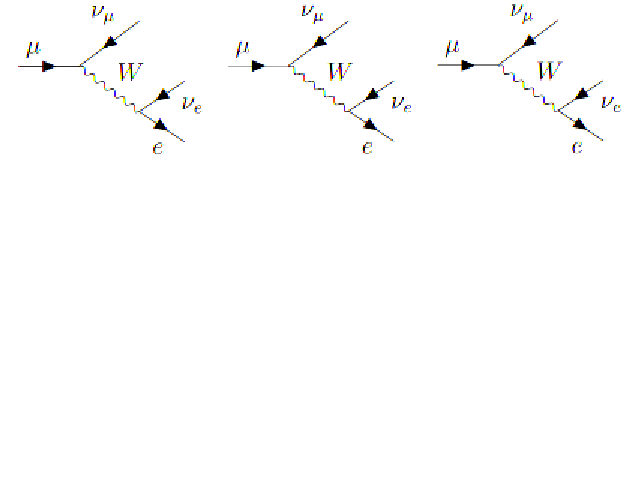
\includegraphics[width=0.5\textwidth]{Figures/5/mu_decay.pdf}
%		 \begin{tikzpicture}
%		 	\begin{feynman}
%		 		\vertex (a1); %mu
%
%		 		\vertex at ($(a1) + (1cm, 0)$) (b1); % decay to W+nu_mu
%				
%		 		\vertex at ($(b1) + (1, 0.75)$) (c1); %nu_mu
%				\vertex at ($(b1) + (1, -0.75)$) (c2); %W
%				
%				\vertex at ($(c2) + (0.75, 0.5)$) (d1); % nu_e
%				\vertex at ($(c2) + (0.75, -0.5)$) (d2); % e
%
%		 		\diagram* {
%		 		  (a1) -- [fermion, edge label=\(\mu\), near start] (b1),
%		 		  (c1) -- [fermion, edge label'=\(\nu_\mu\), near start] (b1) -- [boson, edge label=\(W\)] (c2),
%		 		  (d1) -- [fermion, edge label=\(\nu_e\), near start] (c2) -- [fermion, edge label'=\(e\), near end] (d2),
%		 		};
%		 	\end{feynman}
%		 \end{tikzpicture}
	\caption{Muon decay}
	\label{fig:muon_decay}
	\end{subfigure}
	\begin{subfigure}[t]{0.49\textwidth}
	\centering
	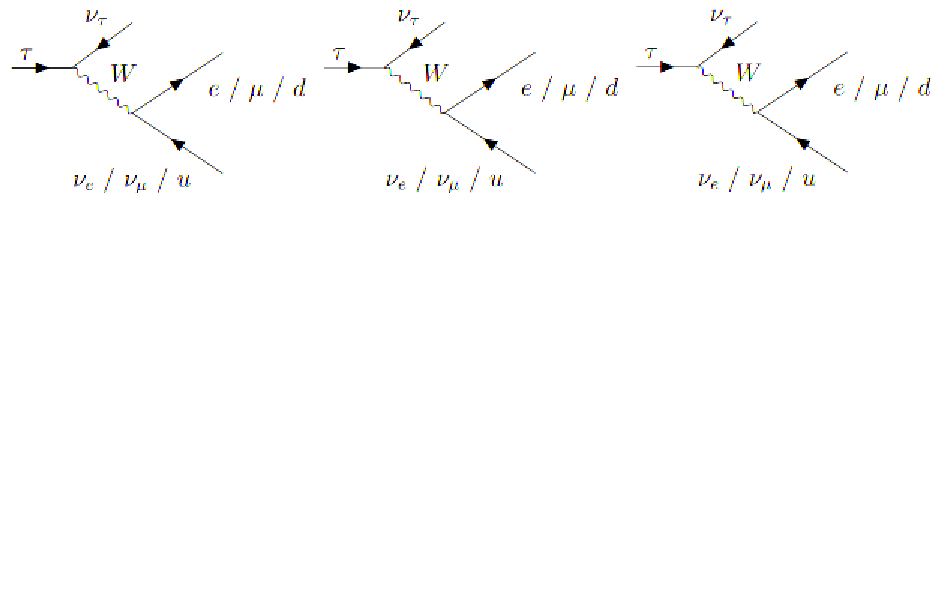
\includegraphics[width=0.75\textwidth]{Figures/5/tau_decays.pdf}
%		 \begin{tikzpicture}
%		 	\begin{feynman}
%		 		\vertex (a1); %tau
%
%		 		\vertex at ($(a1) + (1cm, 0)$) (b1); % decay to W+nu_tau
%				
%		 		\vertex at ($(b1) + (1, 0.75)$) (c1); %nu_tau
%				\vertex at ($(b1) + (1, -0.75)$) (c2); %W
%				
%				\vertex at ($(c2) + (1.5, -1)$) (d1); % nu_e / nu_mu / u / d
%				\vertex at ($(c2) + (1.5, 1)$) (d2); % e / mu / d / u
%
%		 		\diagram* {
%		 		  (a1) -- [fermion, edge label=\(\tau\), near start] (b1),
%		 		  (c1) -- [fermion, edge label'=\(\nu_\tau\), near start] (b1) -- [boson, edge label=\(W\)] (c2),
%		 		  (d1) -- [fermion, edge label={\(\nu_e\) / \(\nu_\mu\) / \(u\)}, near start] (c2) -- [fermion, edge label'={\(e\) / \(\mu\) / \(d\)}, near end] (d2),
%		 		};
%		 	\end{feynman}
%		 \end{tikzpicture}
	\caption{Tau decay}
	\label{fig:tau_decay}
	\end{subfigure}
	\caption{Decay mechanisms for muons and taus}
	\label{fig:lepton_decays}
\end{figure}

Due to their relatively large mass of 1.8 \GeV, taus can decay either leptonically to \(e\bar{\nu}_e\) or \(\mu\bar{\nu}_\mu\), or hadronically to \(d\bar{u}\), as shown in Figure \ref{fig:tau_decay}, and their decays proceed with a much shorter mean lifetime compared with the muon of 0.3ps. Because of this relatively short lifetime, taus will decay before passing through the ATLAS detector, and as such it is their leptonic or hadronic decay products that are actually measured in the detector. As will be discussed in Section \ref{sec:evt_selections} below, the selections applied for this analysis require that events have exactly one electron or muon in the final state in order to be considered for the search. As a result, the search is sensitive to \(s\rightarrow WW\) decays in which the leptonically decaying \(W\) decays to \(\tau\nu_\tau\) only in the case where the \(\tau\) decays leptonically to produce a single energetic electron or muon in the final state, which occurs with a 35\% branching fraction.

\subsubsection{Electrons}

As discussed in Section \ref{sec:EM_calo}, electron objects are reconstructed from clusters of energy deposits in the electromagnetic calorimeter that are associated with tracks in the inner detector, and calibrated to the EM scale. Detailed information about electron reconstruction, identification, and calibration can be found in Refs.~\cite{ATL-PHYS-PUB-2017-022}, \cite{PERF-2017-01} and \cite{PERF-2017-03}. To accommodate the differing needs of the various studies which make use of electron objects, ATLAS reconstructs these objects at several levels of identification and isolation efficiency, where these different efficiency levels are referred to as ``working points", and are typically referred to as variants of \emph{Loose}, \emph{Medium} and \emph{Tight} for reasons that will be discussed in the following paragraphs.

The identification efficiency refers to the probability that an electron passing through the detector will be correctly reconstructed and identified as such. In general, higher efficiency is achieved by loosening electron identification criteria, and comes at the cost of increased background acceptance. Increased background acceptance means that reconstructed objects have a higher probability of being incorrectly identified as having originated from an electron. 

Electron isolation tackles a slightly different, though related, challenge in comparison with identification. The goal of isolation is to separate the so-called ``prompt" electrons that are produced from the primary decay processes of heavy mediators produced in the \(pp\) collisions from background processes such as semileptonic quark decays, hadrons misidentified as leptons and photons that convert into \(e^+e^-\) pairs before reaching the EM calorimeter. It is generally found that reconstructed objects which originate from prompt electrons can be characterized by a relative absence of (i.e. isolation) from significant activity in a small angular radius in \(\eta\times\phi\) around the object. In analogue with the identification efficiency, a high isolation efficiency is achieved by loosening the criteria for defining an object as isolated. As such, prompt electrons have a high probability of being identified as isolated, but comes at the cost of an increased rate of incorrectly identifying objects which originate from background processes as isolated.
 
Two types of electrons are defined for the search based on different sets of criteria:
\newline \emph{Baseline} electrons use the \emph{Loose} working point for both identification and isolation. Isolation is measured within a fixed angular radius of \(\Delta R=0.2\) around the reconstructed electron object \cite{PERF-2017-01}. The \emph{Loose} identification working point is measured in dedicated studies performed within the ATLAS collaboration to have an efficiency of 93\% \cite{PERF-2017-01} for identifying prompt electrons with \(E_T=40~\GeV\). The \emph{Loose} isolation working point has a total measured efficiency of 98\% \cite{PERF-2017-01}. This electron definition has a relatively high efficiency, and is used to veto the presence of additional electrons in the final state.
\newline \emph{Signal} electrons are designed to be high-purity electrons. They are required to satisfy the \emph{Medium} identification criteria, which are measured to have an 88\% efficiency \cite{PERF-2017-01}, and \emph{Loose} isolation criteria.
\newline Both types of electrons require are required to have \(\pT > 7{\GeV} \) and a pseudorapidity in the range of \(|\eta| < 2.47\).

\subsubsection{Muons}

As described in Section \ref{sec:muon_spec}, muons are reconstructed using information from the the inner detector and the muon spectrometer. Detailed information about muon reconstruction, identification and calibration can be found in Refs. \cite{PERF-2015-10} and \cite{ATL-PHYS-PROC-2018-052}. In analogy to electron objects, muon objects are reconstructed at several identification and isolation working points, and two definitions for muons are considered for this analysis:
\newline \emph{Baseline} muons do not have any isolation requirement, and must satisfy the \emph{Loose} identification criteria, with a measured efficiency of 98\% for \(20~\GeV<p_{T, \mu}<100~\GeV\) \cite{PERF-2015-10}, for a high-efficiency selection.
\newline \emph{Signal} muons are designed to have a relatively high purity, and must satisfy the \emph{Medium} identification criteria, with a 98\% efficiency for \(20~\GeV<p_{T, \mu}<100~\GeV\) \cite{PERF-2015-10}. Signal muons are additionally required to pass a set of tight isolation criteria referred to as \emph{TightTrackOnly\_VarRad} \cite{ATL-PHYS-PROC-2018-052} which use information from the inner tracker, and are defined within an angular radius \(\Delta R\) around the reconstructed muon object that depends on the \pt of the muon object.
\newline Both types of muons use a threshold of \(\pt > 7~\GeV \). 

Baseline muons are required to have pseudorapidity in the range of  \(|\eta| < 2.7\). For signal muons, a tighter pseudorapidity range of \(|\eta| < 2.5\) is required to ensure that the muons are well measured in the inner detector as well as the muon spectrometer. 

\subsection{Small-radius \aktfour jets}
\label{sec:atk4_jets}

As discussed in detail in Section \ref{sec:had_calo}, quarks and gluons hadronize in the hadronic calorimeter to produce showers of energy deposits in the calorimeter known as jets. This search uses the ``particle flow algorithm" \cite{PERF-2015-09} to reconstruct objects associated with the resulting energy deposits. The particle flow algorithm matches signals from the inner tracker and the topologically connected clusters of energy deposits in the calorimeter referred to as ``topo-clusters" with the aim of forming objects representing individual charged particles. The energy deposited in the calorimeter by these identified charged particle objects is, leaving behind an ensemble of ``particle flow objects" consisting of the remaining calorimeter energy and tracks which are matched to the hard interaction. The anti-\(k_t\) algorithm described in Ref. \cite{akt_algo} is then used to reconstruct jets using these particle flow objects. Various angular jet radii \(R\), where \(R\) is defined in Eq. \ref{eq:jet_radius}, may be considered for jet reconstruction depending on the kinematics and anticipated origins of the quark or gluon which initiated the shower (see discussion in Section \ref{sec:had_calo} for more details), where \(R\) determines the angular radius within which the anti-\(k_t\) algorithm includes calorimeter deposits for jet reconstruction. 

As discussed in Chapter \ref{chapter:dh_model}, the final state signature of DH model targeted in this search involves a pair of energetic \(W\) bosons in the final state, one of which decays leptonically to a \(\ell\nu\) pair, and the other hadronically to a pair of quarks. If the boost of the hadronically decaying \(W\) is sufficiently low, the two quarks may have a large enough angular separation as to be most effectively reconstructed as two separate jets with small radius. In the so-called ``resolved" regime of the search, the quark-induced jets so resolved that it is not even possible to reconstruct them as a single multi-pronged large-radius jet. For this search, these so-called ``\smallR" jets are reconstructed with a radius of \(R=0.4\).

After the \smallR jets are reconstructed are fully calibrated \cite{ATLAS-CONF-2015-037}, only jets with \(\pt > 20~\GeV\) and \(|\eta| < 2.5\) are considered for the search. Jet cleaning \cite{ATLAS-CONF-2015-029} with the \emph{TightBad} working point is applied to suppress noise in the calorimeter and background jets which are not produced from the primary \(pp\) collision. The jet vertex tagger \cite{ATLAS-CONF-2014-018} is applied with the \emph{Tight} working point to suppress pileup jets \cite{pileup} from other \(pp\) interactions in the same and neighbouring bunch crossings - see Section \ref{sec:evt_wts} for a more detailed discussion of pileup events. As described in Section \ref{sec:resolved_w_cand} below, these jets are used in the analysis to identify quarks originating from the hadronically-decaying \(W\) boson in the DH signal model in the resolved regime, and to reconstruct the \(W\) boson in this regime.

\subsubsection*{\btag}
\btagged jets are identified with the \verb|DL1r| algorithm \cite{ATLAS-CONF-2018-006}, which uses a deep learning method for the identification. A fixed working point with 77\% efficiency is used. \btagged jets are vetoed in the signal region to reduce the background of SM \ttbar and single-top processes (see Section \ref{sec:dominant_bkgs} for details).

\subsection{Resolved \(W\) Candidate}
\label{sec:resolved_w_cand}

As described in Section \ref{sec:atk4_jets} above, the pair of quarks produced by the hadronic decay of the \(W\) boson in the signal model are reconstructed as two resolved \smallR jets in the less-boosted resolved regime. The parent \(W\) boson can then be reconstructed from \smallR jets induced by its daughter quarks using the combined energy and momentum of the \smallR jet pair. Given that \smallR jets can also be produced by, for example, initial-state radiation and pileup, it is quite common for there to be more than two \smallR jets reconstructed in the final state. These additional \smallR jets introduce some ambiguity in terms of identifying which \smallR jets reconstructed in the final state should be associated with the hadronic decay of a \(W\) in the signal model. For events with more than two \smallR jets in the final state, the pair of \smallR jets whose combined invariant mass is closest to the \(W\) boson mass are associated with the \(W\) decay products, and used to reconstruct the \(W\) boson candidate. The algorithm for this jet identification and \(W\) boson reconstruction so is as follows:

\begin{itemize}
\item Construct all possible combinations of two \smallR jets (a.k.a. ``dijet pairs") in the final state.
\item For each such candidate dijet pair, \(j_1\) and \(j_2\), sum the four-momenta of the reconstructed jets, \(\mathbf{p}_{j_1,j_2} = \mathbf{p}_{j_1} + \mathbf{p}_{j_2}\), and calculate their combined invariant mass: 

\begin{equation}
\label{eq:dijet_invt_mass}
M_{j_1,j_2} = \sqrt{\mathbf{p}_{j_1,j_2} \cdot \mathbf{p}_{j_1,j_2} } 
\end{equation}
\item Select the dijet pair whose invariant mass is closest to the \(W\) boson mass of \(80.4~\GeV\) \cite{PDG_2018} as the \smallR jets to be associated with the \(W\rightarrow q\bar{q}\) decay.
\item Reconstruct the candidate hadronically decaying \(W\) boson using the dijet pair with four-momentum \(\mathbf{p}_{j_1,j_2}\).
\end{itemize}

Figure \ref{fig:resolved_Wmass_reco} shows distributions of the reconstructed mass of the \(W\) boson candidate for MC simulated events generated at a range of sample \ms and \mZp after application of the baseline event selections presented in Section \ref{sec:evt_selections}, with the additional requirement that there be at least two \smallR jets in the final state. The distributions are in general well centred around the \(W\) boson mass.

\begin{figure}[h]
	\centering
	\begin{subfigure}[b]{0.49\textwidth}
	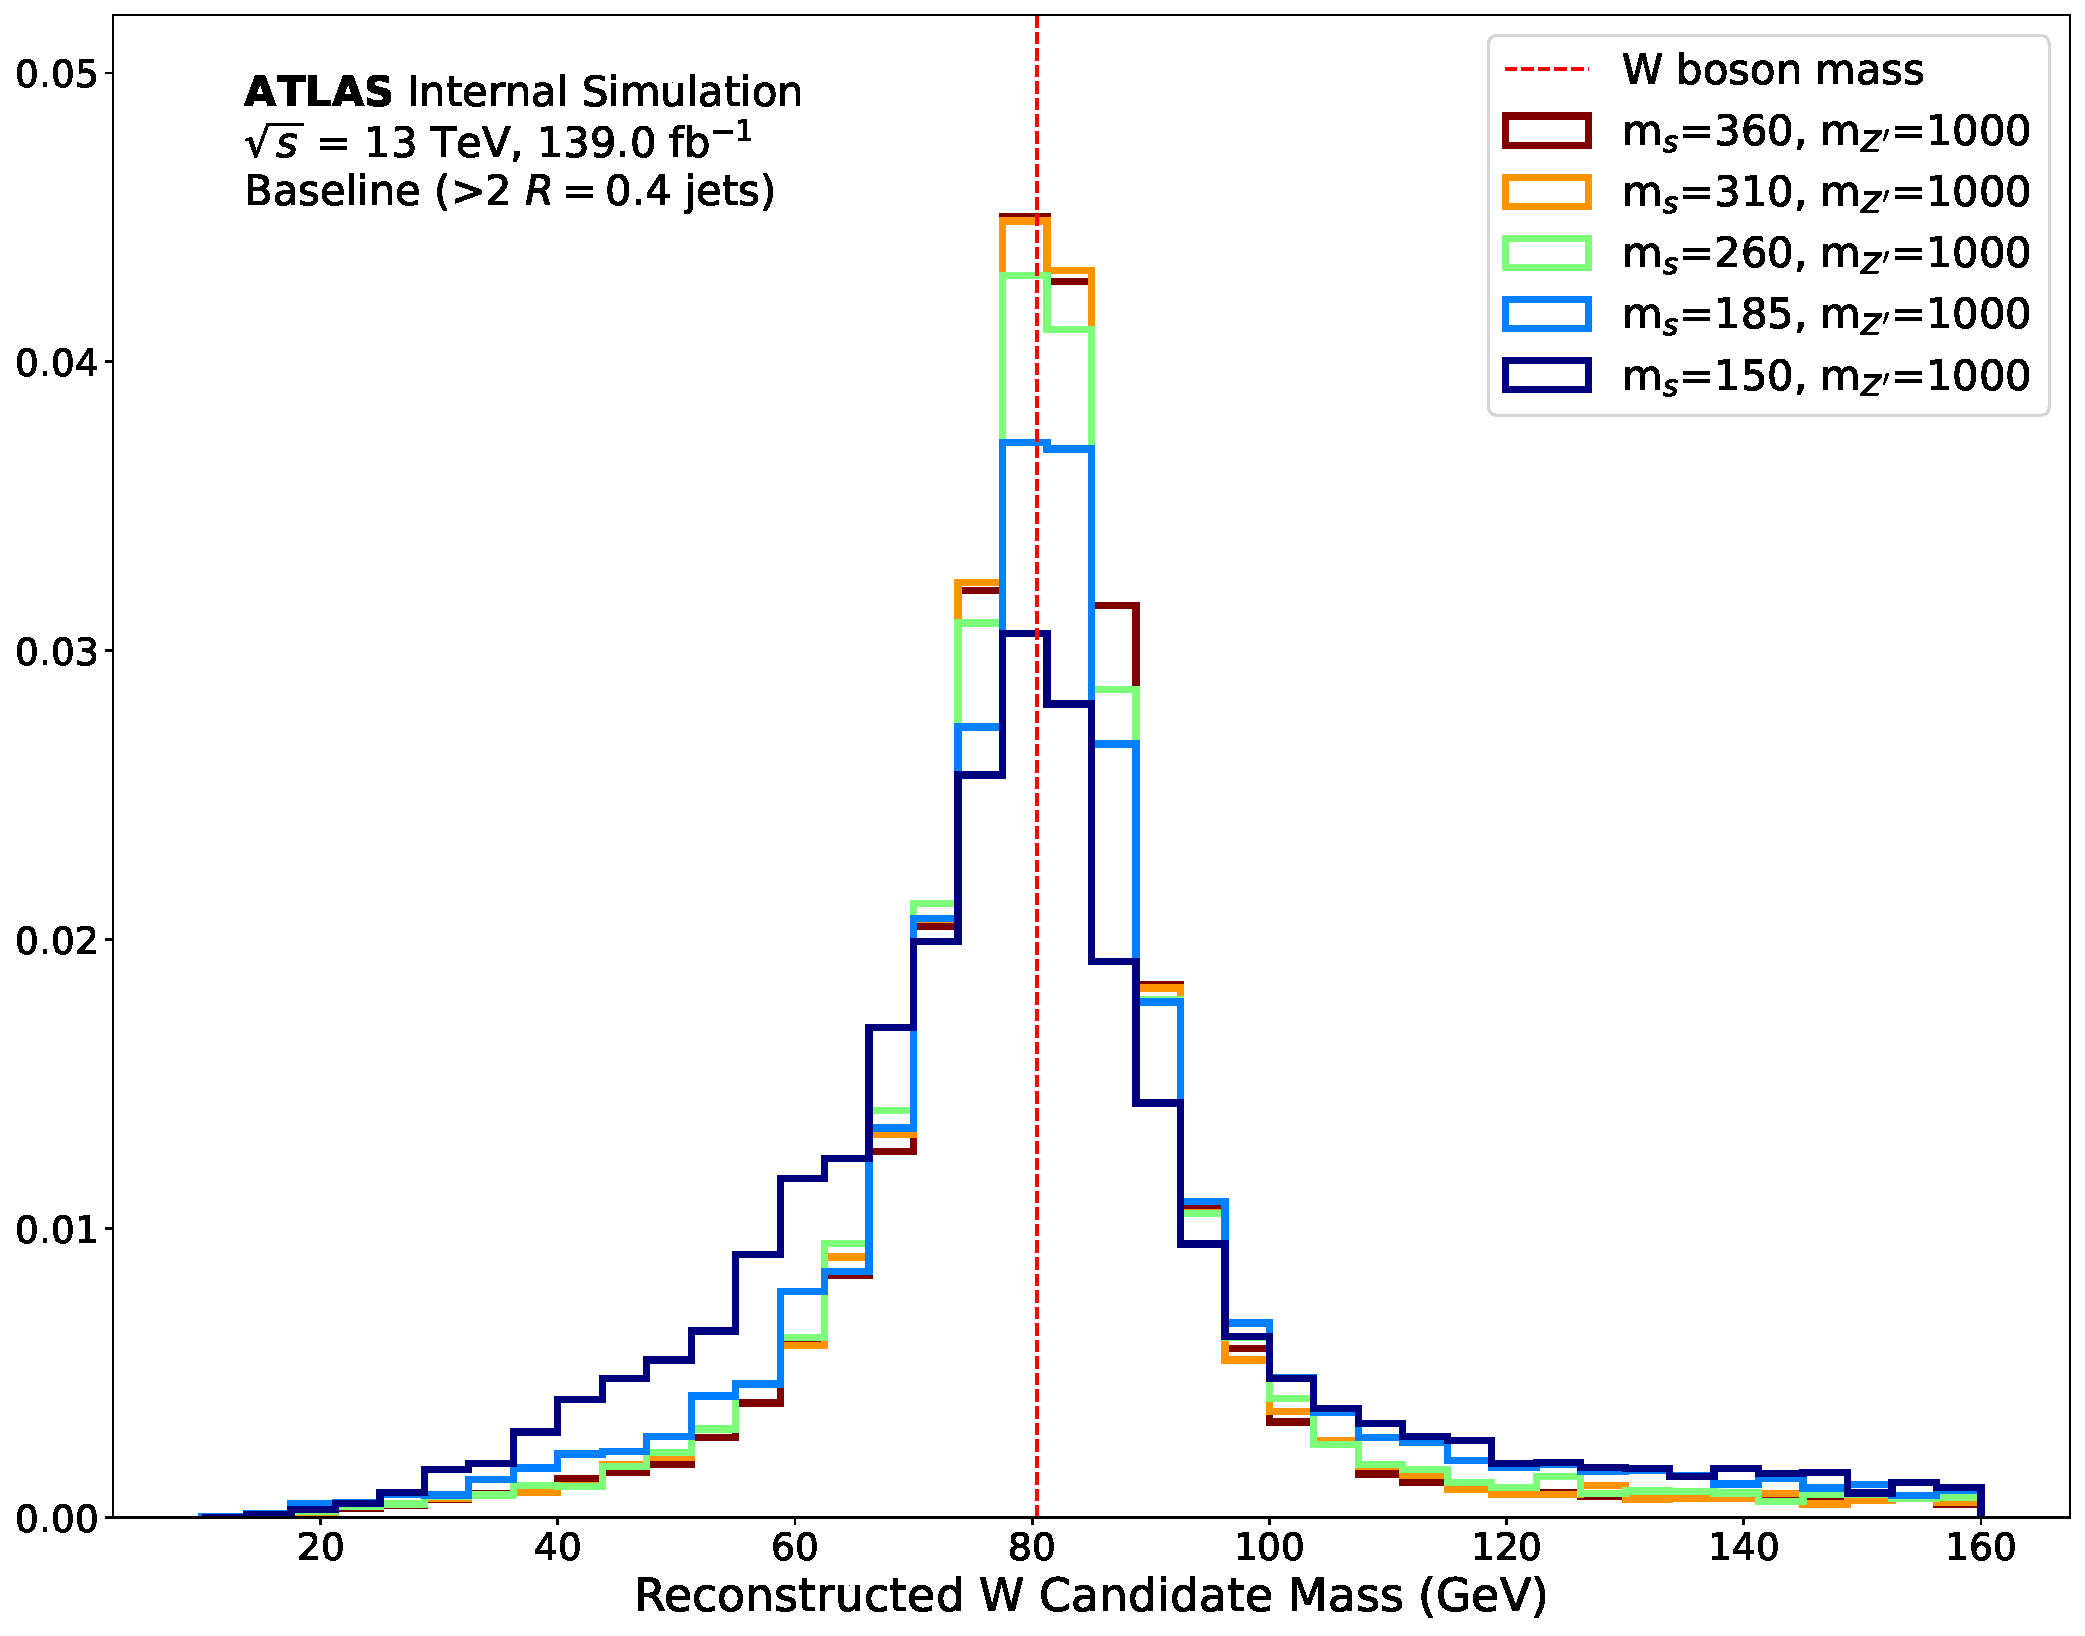
\includegraphics[width=0.95\textwidth]{Figures/5/WCand_m_ms.pdf}
	\caption{\mZp Fixed, \ms Varied}
	\label{fig:resolved_Wmass_reco_ms}
	\end{subfigure}
	\begin{subfigure}[b]{0.49\textwidth}
	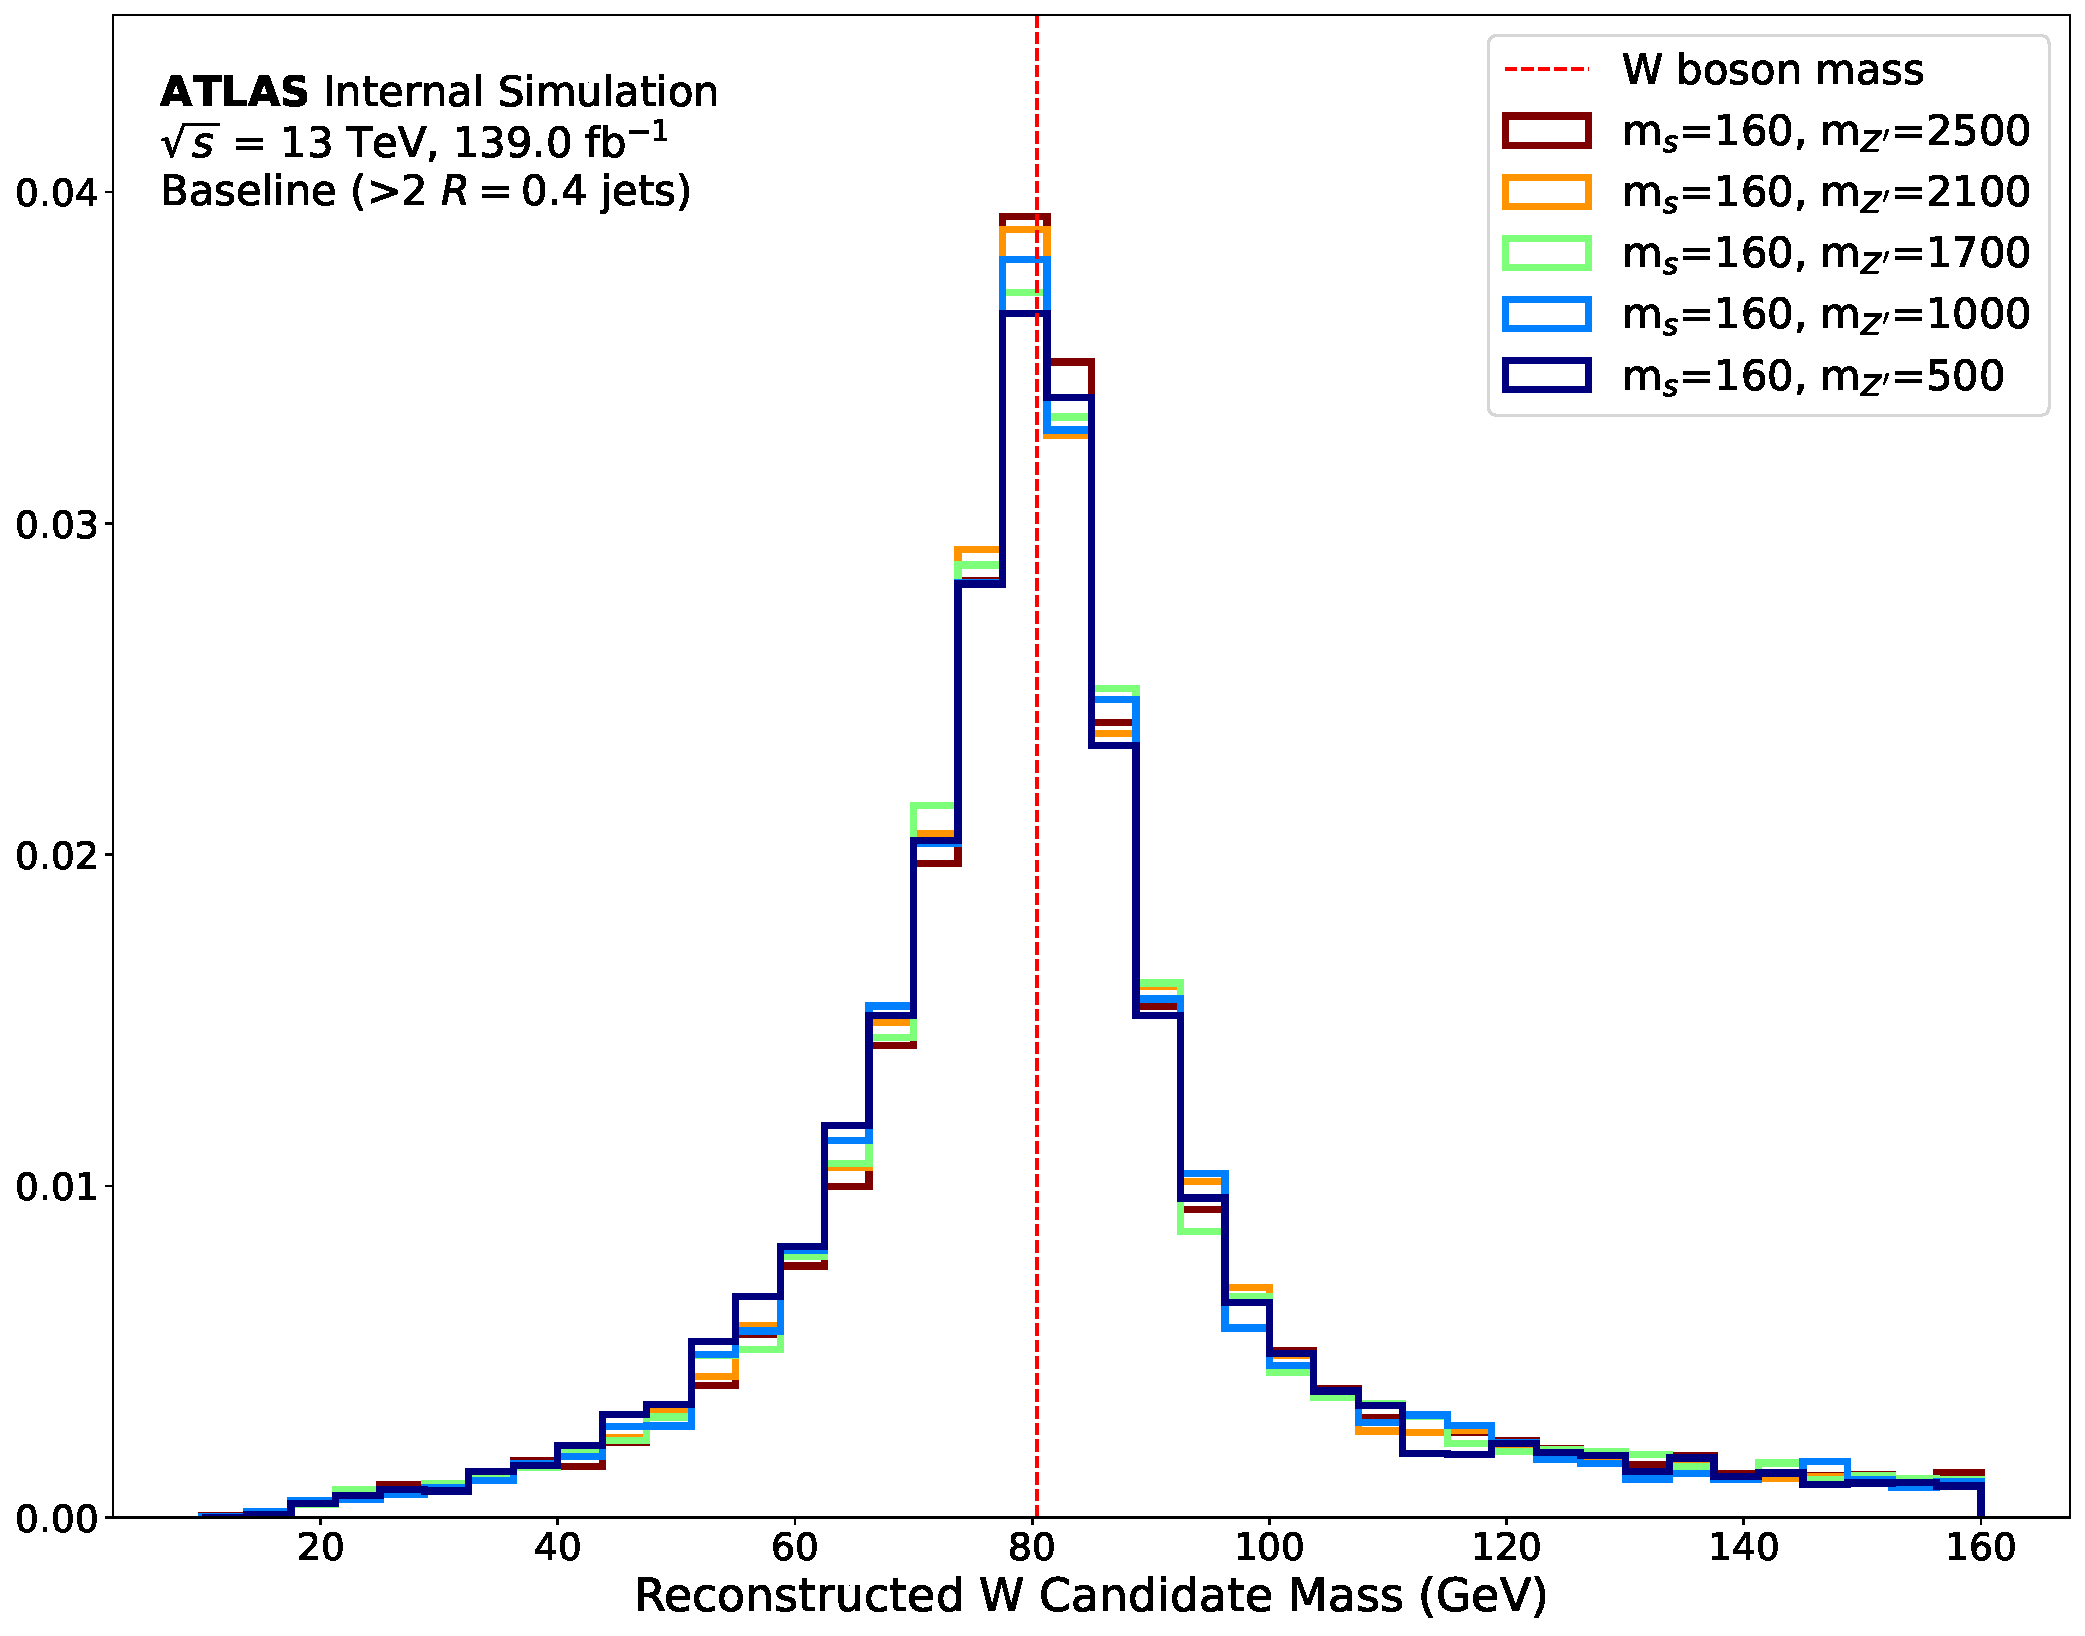
\includegraphics[width=0.95\textwidth]{Figures/5/WCand_m_mZp.pdf}
	\caption{\ms Fixed, \mZp Varied}
	\label{fig:resolved_Wmass_reco_mZp}
	\end{subfigure}
	\caption[]{Distributions of the reconstructed W candidate mass for MC simulated events produced for the DH signal model over a range of \ms and \mZp. All events included in the distributions are required to pass the baseline event selection described in Section \ref{sec:evt_selections} is applied, and to have at least two \smallR jets in the final state. The red dashed vertical line is placed at the \(W\) boson mass of 80.4 \GeV. Note that the differing amplitudes of the distributions are largely due to differing cross sections of the DH signal model at the different \ms and \mZp plotted.}
	\label{fig:resolved_Wmass_reco}
\end{figure}

\subsection{Track-Assisted Reclustered Jets (Merged \(W\) Candidate)}
\label{sec:TAR_jets}

If the hadronically decaying \(W\) boson is produced with a sufficiently large momentum (i.e. boost), the jets produced by the \(q\) pair may be sufficiently collimated (i.e. ``merged") that they are most effectively reconstructed as a single multi-pronged large-radius jet, as opposed to the resolved \smallR jets used for \(W\) reconstruction in the resolved regime (see Sections \ref{sec:atk4_jets} and \ref{sec:resolved_w_cand} above for details). 

Since the signal model predicts that charged particle tracks and energy deposits in the detector will have originated primarily from the two quarks produced by the \(W\rightarrow q\bar{q}\) decay in the signal model, it is important to reconstruct the large-radius jet in this so-called merged regime with as much detailed kinematics and substructure information as possible, in order to identify features that would be consistent with the jet containing tracks and energy deposits originating from two energetic quarks originating from a \(W\) parent. Such features would include the combined invariant mass \mTAR of all particles which produced the jet, which would be expected to be consistent with the \(W\) boson mass within detector resolution. Important substructure information would include variables which aim to quantify the number of distinct ``prongs" of localized energy deposition within the jet, which can be correlated to the number of high-\pt strongly interacting particles whose energy deposits are included in the jet (two such prongs would be expected for the signal model). 

This search uses the track-assisted reclustered (TAR) jet algorithm \cite{ATL-PHYS-PUB-2018-012} for large-radius jet reconstruction in the merged regime. In this regime, the highest-\pt TAR jet reconstructed with a radius parameter of \(R=1.0\) is identified as the physics object which constitutes the the decay products of the candidate hadronically decaying \(W\) boson (\(W_\text{had}\)) in the DH signal model. Whereas most large-radius jet reconstruction techniques rely on energy deposits in the calorimeter to construct the jet substructure information, TAR jets are designed to combine charged particle tracks measured by the inner tracker with the calorimeter energy deposits to obtain a higher-resolution construction of TAR substructure information, taking advantage of the superior resolution of the inner tracker compared with calorimeter. 

\subsubsection{TAR Algorithm}
\label{sec:TAR_algo}

For this search, \(R=0.2\) \smallR jets are used to reconstruct energy deposits in the calorimeter, and are input to the TAR algorithm along with tracks measured by the inner detector which satisfy a set of quality criteria summarized in Table \ref{tab:TARparameters}. The TAR algorithm \cite{ATL-PHYS-PUB-2018-012} is as follows: the input \(R=0.2\) \smallR ``subjets" are reclustered using the \akt algorithm with \(R=1.0\) to \largeR jets. A trimming procedure is applied to mitigate the effects of pileup and background QCD processes within the triggered event that do not originate from the hard interaction. The trimming procedure removes any of the input subjets which carry less than a fraction \(\fcut=0.05\) of the total transverse momentum of the \largeR jet: \(\pt^\text{subjet}/\pt^\text{\largeR jet} < 0.05\).  The tracks from the inner detector are then matched to the remaining \smallR subjets using the ghost association procedure described in Ref. \cite{ghost_association_2008}, if possible. Any tracks which cannot be matched to subjets using ghost association are instead matched to the nearest subjet, provided that there is a jet within an angular radius \(\Delta R=0.3\) of the track. To account for the energy of the neutral hadronic jet components which do not leave tracks in the inner detector, the \pt of each track is scaled such that the \(\pt\)s of all tracks matched to a given subjet will sum to the energy of the subjet measured by the calorimeter:

\begin{equation}
\label{eq:tar_track_pt_scaling}
\pt^\text{track, new} = \pt^\text{track, old} \times \frac{p_{T,j}^\text{subjet}}{\sum_{i \in j}p_{T, i}^\text{track, old}}
\end{equation}

\noindent where the index \(i\) runs over all tracks matched to the subjet \(j\). The rescaled tracks and remaining subjets are again reclustered using the \akt algorithm to form the final \largeR TAR jet.

While the kinematic properties of the TAR jets are calculated from the constituent \smallR jets, the jet substructure as well as the mass \(m^\text{TAR}\) are calculated from the constituent tracks. Figure \ref{fig:TARAlg} shows a visual summary of the basic TAR algorithm. 

\subsubsection{TAR-lepton Disentanglement}

The analysis uses the TAR algorithm on \(R=0.2\) \smallR jets and tracks that have undergone a ``TAR-lepton disentanglement" preselection to remove tracks associated with any reconstructed baseline electrons or muons and any \(R=0.2\) jets which overlapped with the baseline electron tracks. This preselection is helpful in this analysis because the charged lepton produced by the leptonic \(W\rightarrow \ell\nu\) decay often falls within the \(R=1.0\) cone of the TAR jet, as illustrated in Figure \ref{fig:TAR_lepton_overlap_illustration}, and disrupts the jet reconstruction, particularly by means of additional jet energy induced by calorimetric clusters created by an overlapping electron.

\begin{figure}[H]
  \centering
     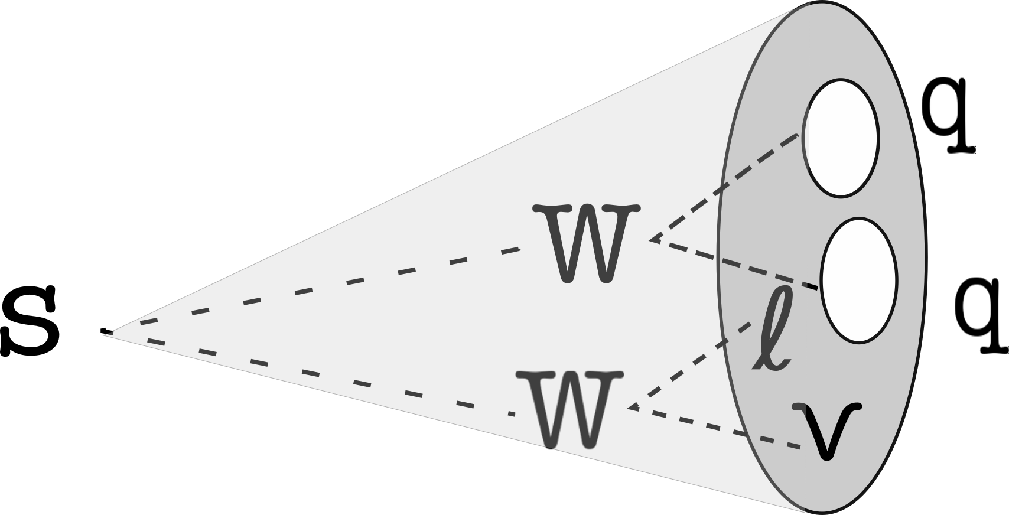
\includegraphics[width = 0.3\textwidth]{Figures/5/lepton_overlap.pdf}
     \caption{Illustration of the final state scenario in which the charged lepton produced by the leptonic \(W\rightarrow \ell\nu\) decay overlaps with the \largeR TAR jet reconstructed from the hadronic \(W\rightarrow qq\) decay.}
     \label{fig:TAR_lepton_overlap_illustration}
  \end{figure}
  
Figure \ref{fig:TARdisentaglementplots} shows a comparison of the distributions of reconstructed TAR jet mass \mTAR either without or with the TAR-lepton disentanglement preselection applied, for MC simulated events produced for the DH signal model at several representative \ms and \mZp, in which the reconstructed electron in the final state overlaps with the highest-\pt reconstructed TAR jet.  An additional requirement on the ``transverse mass" \(m_T\) between the lepton and the \met (see description in Section \ref{sec:transverse_mass} below) if \(\mtlepmet > 150~\GeV\) is applied to select for events with similar kinematics to those which pass the signal region selection presented in Section \ref{sec:evt_selections} below. For all the signal points, the TAR-lepton disentanglement preselection is found to substantially improve the ability of the TAR algorithm to reconstruct TAR jets with \mTAR near the \(W\) boson mass, as would be expected for the signal model.

\begin{figure}[H]
\centering
   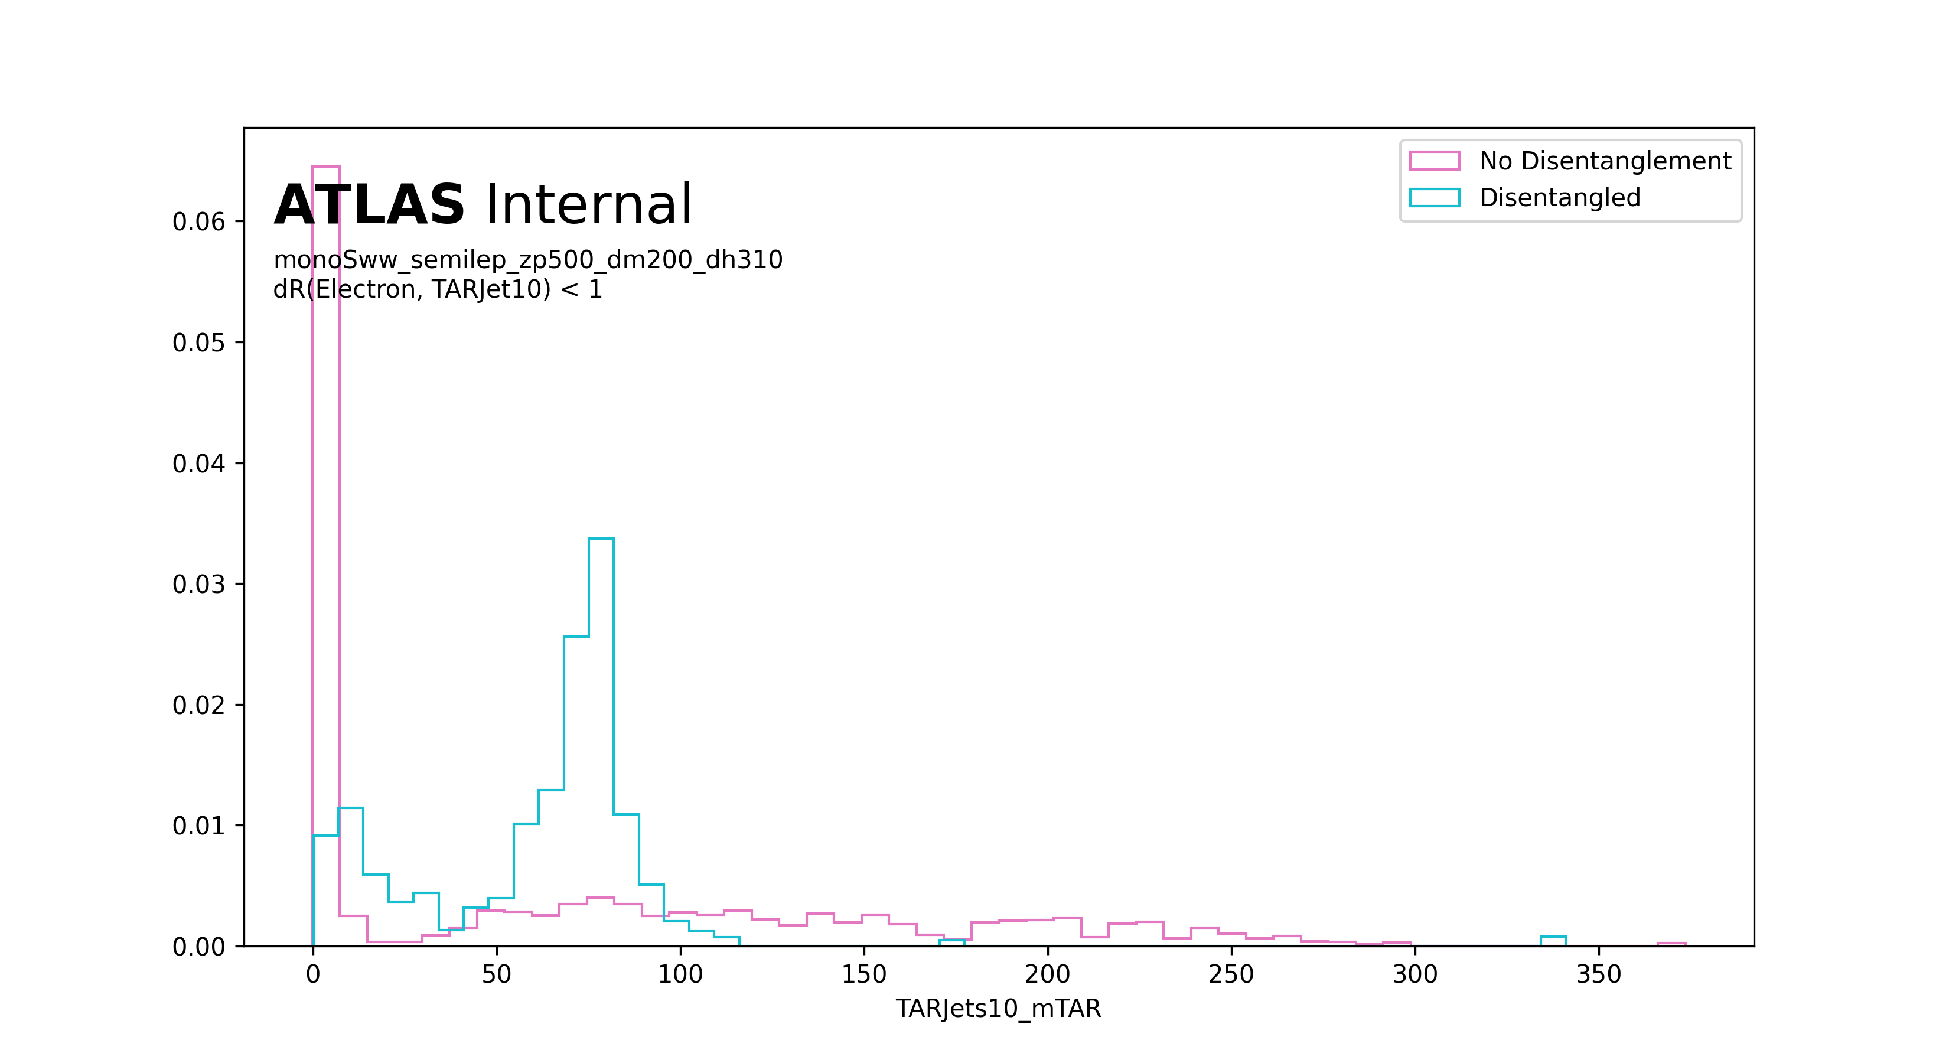
\includegraphics[width = 0.49\textwidth]{Figures/5/monoSww_semilep_zp500_dm200_dh310.pdf}
   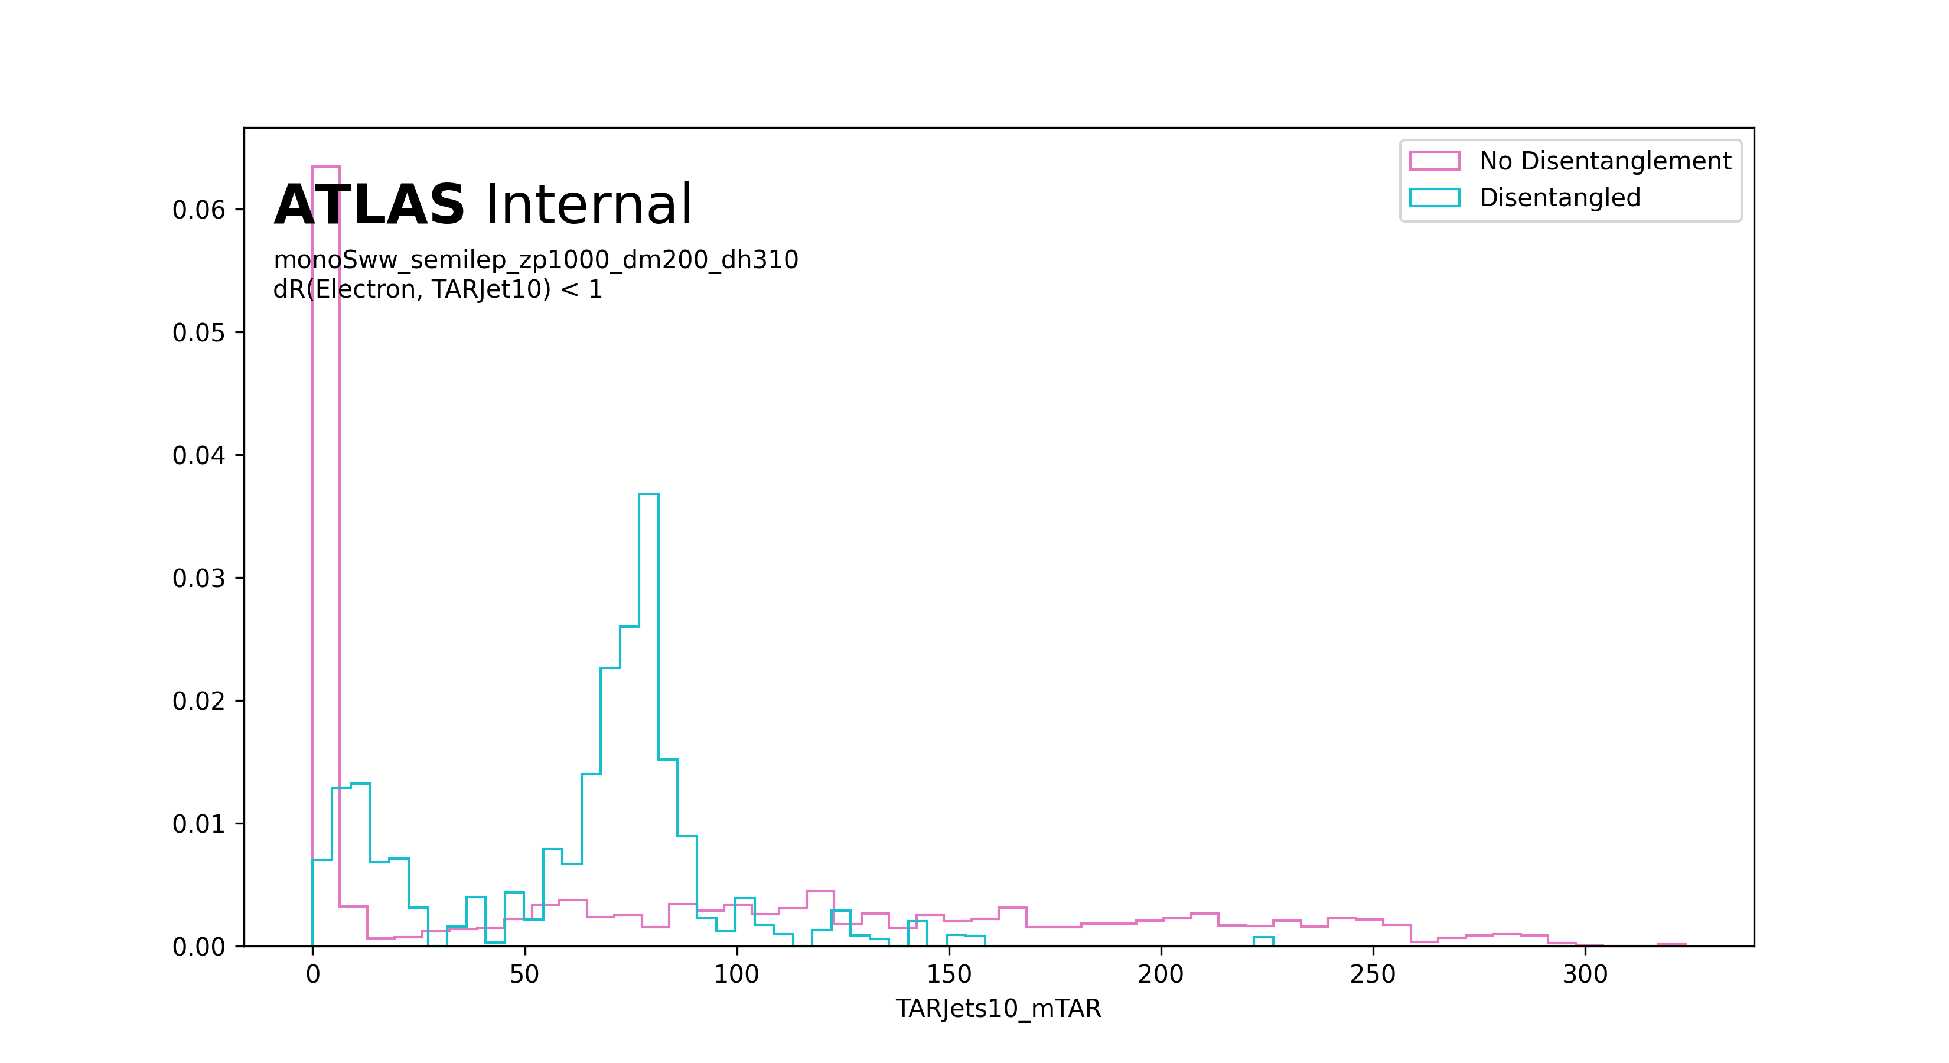
\includegraphics[width = 0.49\textwidth]{Figures/5/monoSww_semilep_zp1000_dm200_dh310.pdf}

   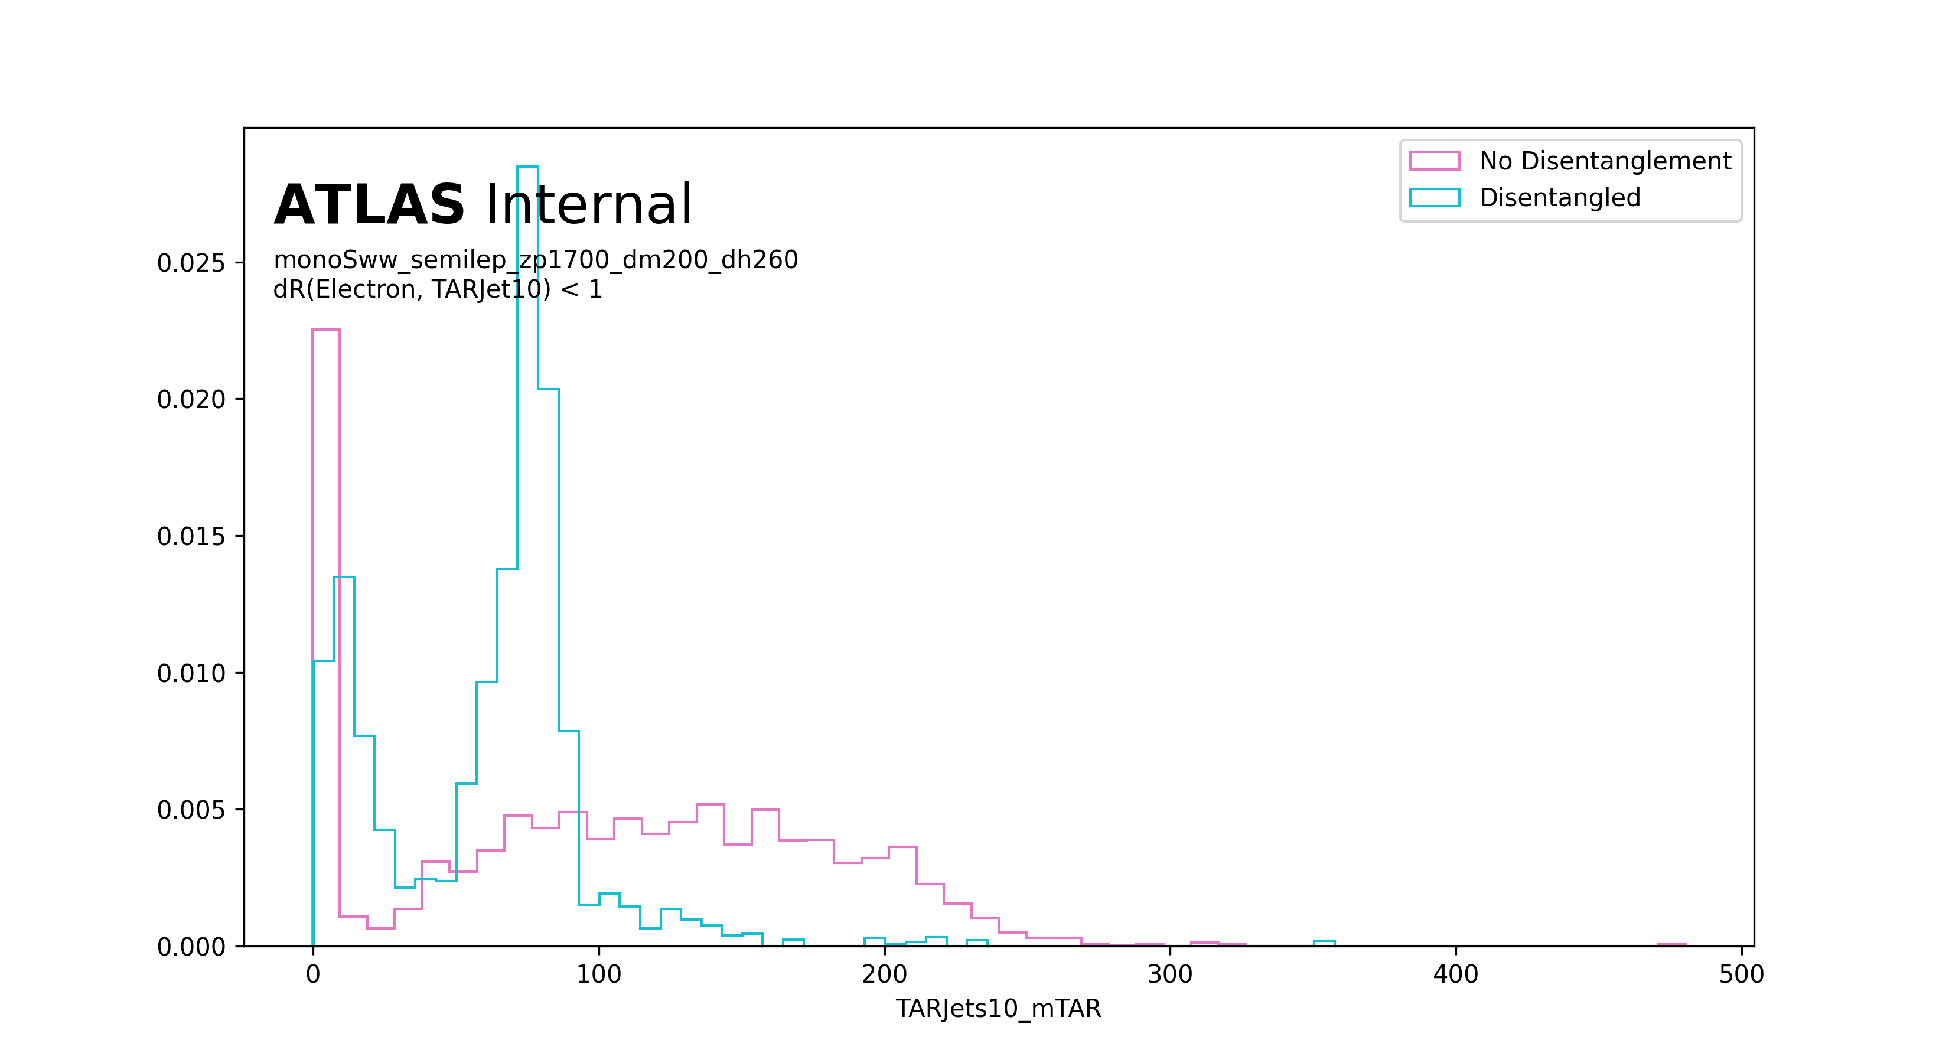
\includegraphics[width = 0.49\textwidth]{Figures/5/monoSww_semilep_zp1700_dm200_dh260.pdf}
   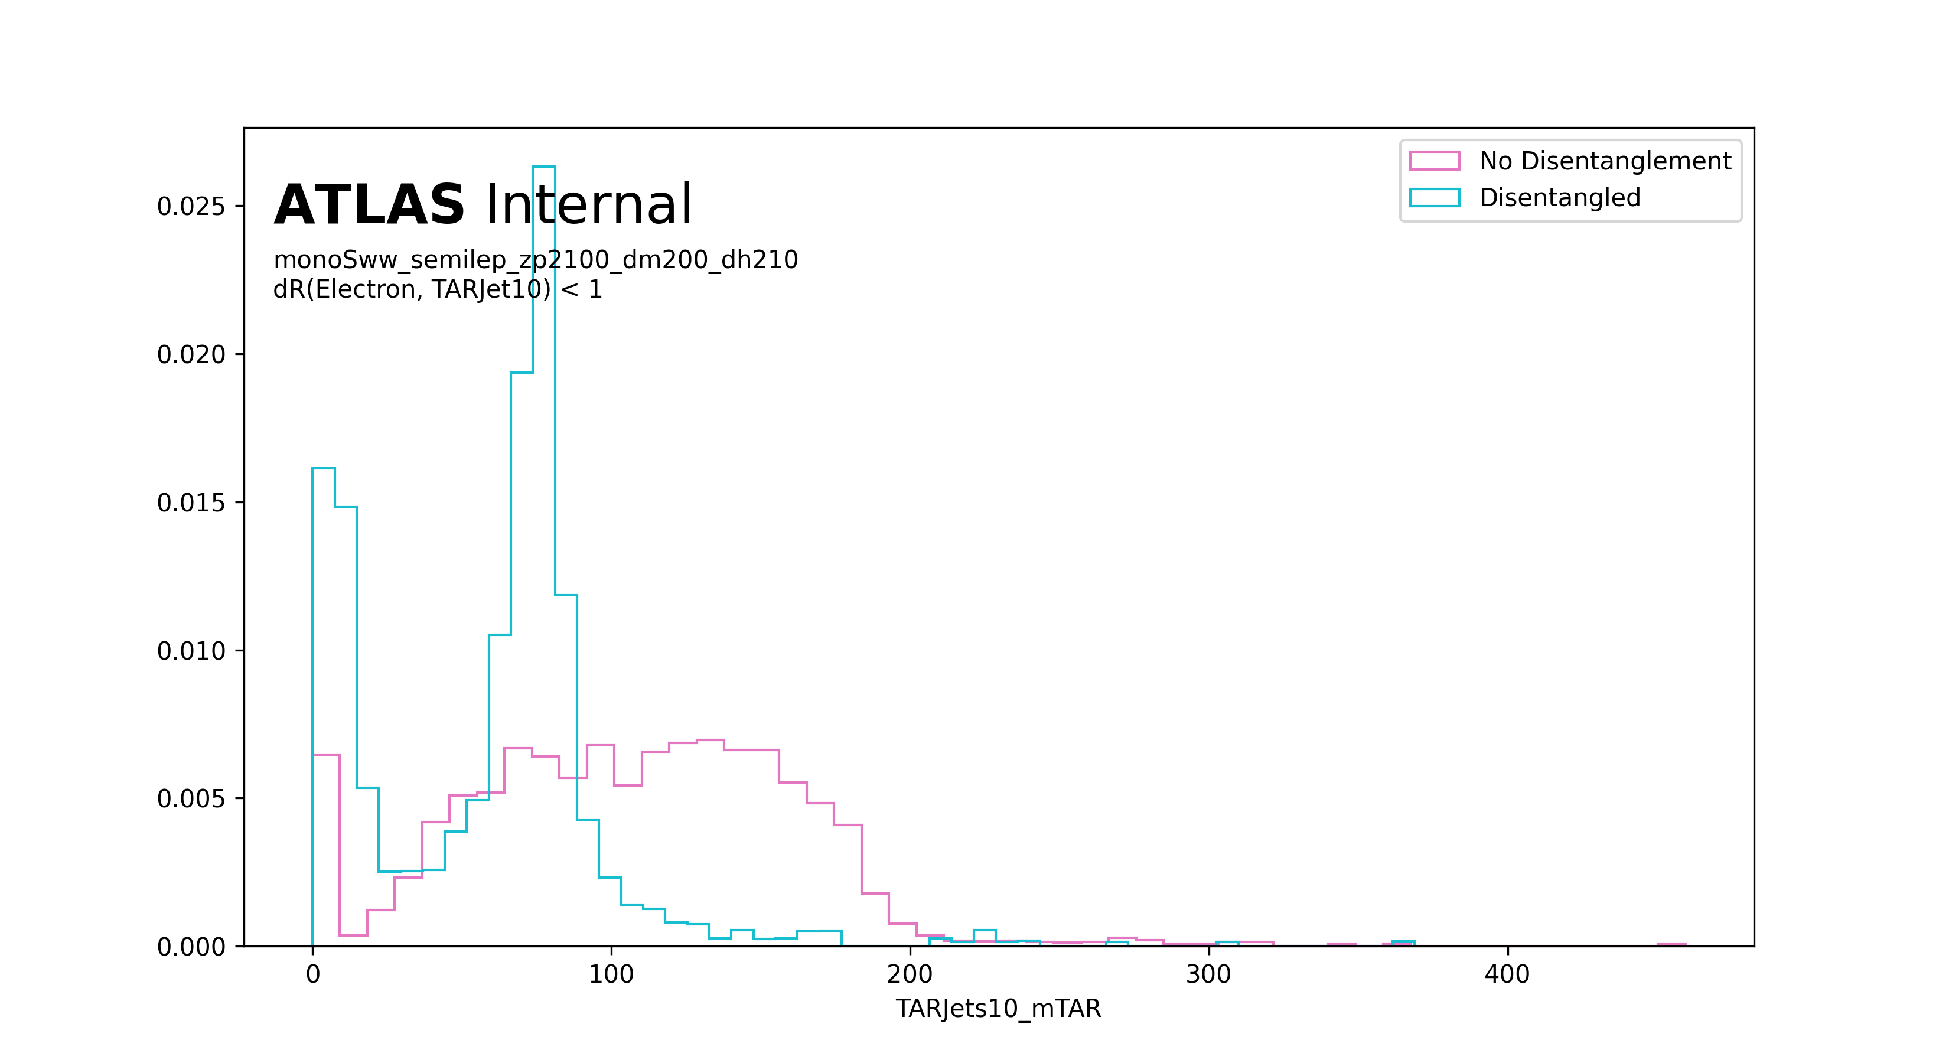
\includegraphics[width = 0.49\textwidth]{Figures/5/monoSww_semilep_zp2100_dm200_dh210.pdf}

   \caption{Distributions of \mTAR for the leading-\pt TAR jet in MC simulated events generated for the DH signal model process with semileptonic \(WW\) decay at several representative \ms and \mZp, with and without application of the lepton disentanglement preselection. Events included in the distributions are required to have one signal electron and at least one reconstructed TAR jet, as well as \(\mtlepmet > 150~\GeV\). Distributions are normalized to unit area.}
   \label{fig:TARdisentaglementplots}
\end{figure}

\subsubsection{Summary of the TAR Procedure}

The following steps summarize the algorithm used to construct the TAR jets used in this search (steps with a * are added to disentangle leptons):
\begin{itemize}
  \item Tracks and calibrated \akt \(R=0.2\) jets are chosen as input to the algorithm.
  \item Tracks associated with a baseline muon or electron are removed from the input collection (*).
  \item \(R=0.2\) jets overlapping with a baseline electron (\(\DeltaR<0.2\)) are removed from the input collection to the TAR algorithm (*).
  \item The remaining \(R=0.2\) subjets are reclustered using the \akt algorithm into \(R=1.0\) jets and trimmed using the \(p_T\) fraction \(\fcut=0.05\).
  \item Input tracks are matched to \(R=0.2\) subjets which remain after trimming, if possible, using ghost association.
  \item Tracks which remain unassociated are matched to the nearest \akt \(R=0.2\) jet within \(\DeltaR<0.3\).
  \item The \pt of each track is rescaled using the \pt of the jet to which it is matched using Eq. \ref{eq:tar_track_pt_scaling}. This rescaling accounts for the missing neutral momentum, which is measured at calorimeter level but is not present at tracker level.
  \item Finally, jet substructure variables and  \(m^\text{TAR}\) are calculated using the rescaled matched tracks.
\end{itemize}
The parameters of the TAR algorithm used are summarized in Table \ref{tab:TARparameters}. \\

\begin{figure}[htb]
  \centering
     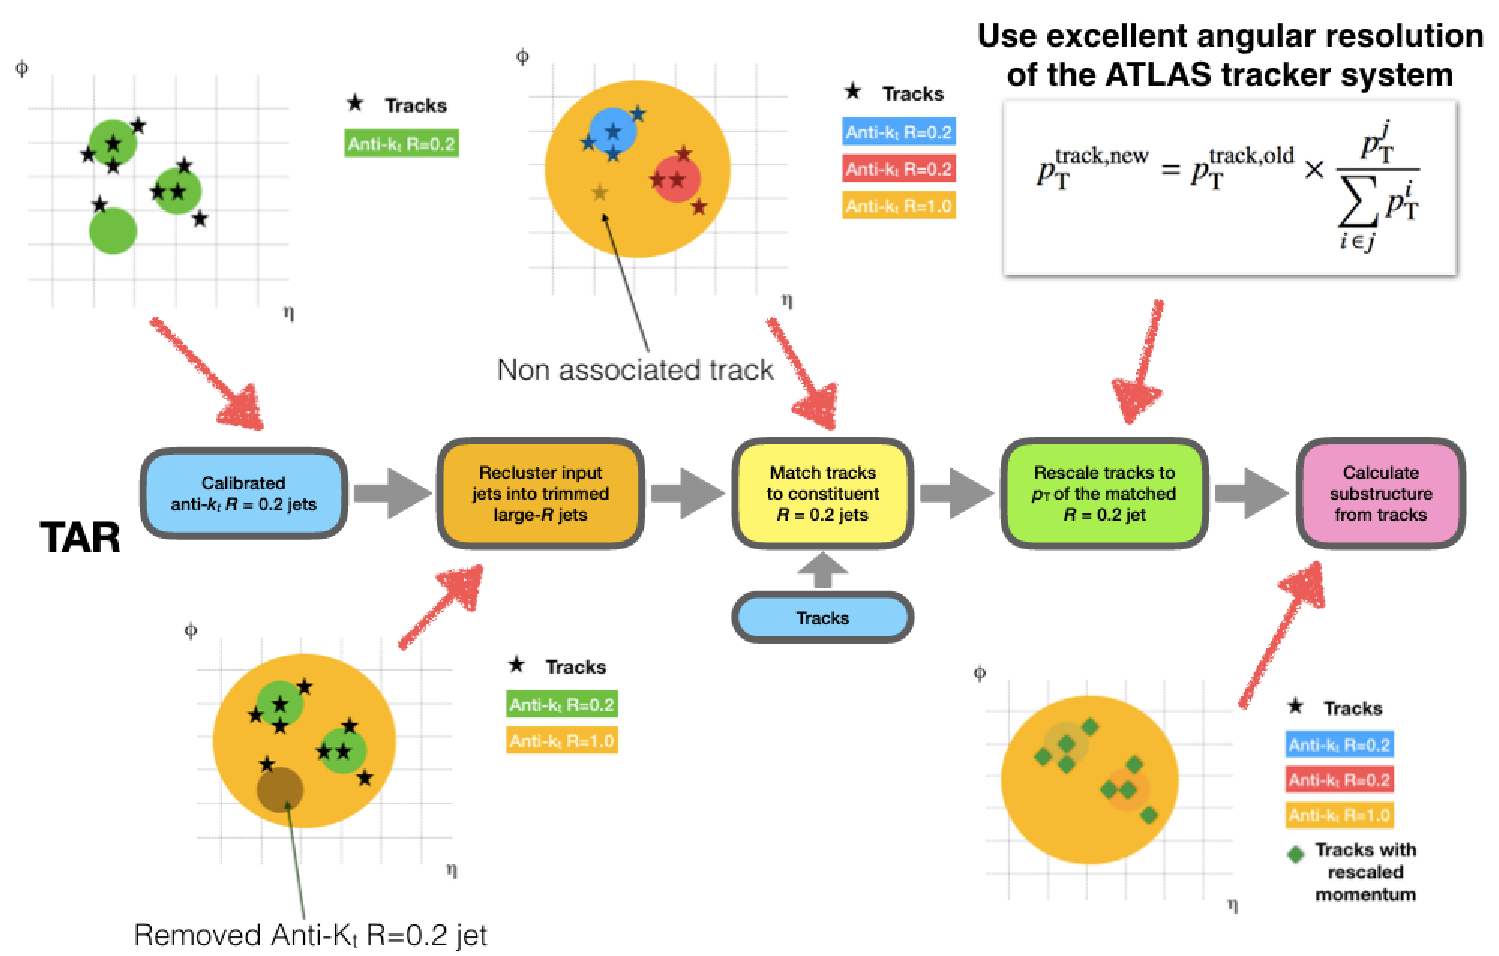
\includegraphics[width = 0.80\textwidth]{Figures/5/TARJetdescription.pdf}
     \caption{TAR jet reconstruction algorithm depicted without lepton disentanglement. Figure adapted from \(\copyright\) \cite{ATL-PHYS-PUB-2018-012}}
     \label{fig:TARAlg}
  \end{figure}

\begin{table}[htbp]
\centering
\caption{TAR jet reconstruction parameters}
\label{tab:TARparameters}
\begin{tabular}{l l }
\toprule
\multirow{3}{*}{Track selection} & \verb|Loose| quality\\
	& \(\pt > 0.5~\GeV\) \\
	& \(|\eta| < 2.5\)  \\
Tracks removed if associated to & electrons, muons \\
\midrule
\multirow{3}{*}{Input jet selection} & \(R=0.2\) \akt jets \\
	& \(\pt > 20~\GeV\) \\
	&  \(|\eta| < 2.5\)  \\
\midrule
Reclustering radius & \(R=1.0\) \\
TAR jet \pt & \(\pt^\text{TAR} > 100~\GeV\) \\
Trimming radius & \(R=0.2\) \\
Trimming \pt fraction & \(f_\text{cut}=0.05\) \\
Track-to-jet association & \(\DeltaR(\text{jet, track}) < 0.3\) \\
jet-electron overlap removal & \(\DeltaR(\text{jet, electron}) < 0.2\) \\
\bottomrule
\end{tabular}
\end{table}

\subsection{\met}

The missing transverse momentum \met, introduced in Section \ref{sec:met}, quantifies the imbalance of momentum in the plane transverse to the beam line. If all particles produced in a \(pp\) collision are fully detected, conservation of momentum implies that the transverse momenta of all objects produced by the event should sum to zero within detector resolution. As a result, large \met in an event is indicative of the production of undetected energetic particles. The semileptonic \(s\rightarrow WW(qq\ell\nu)\) decay channel of the LHC signature for the DH model probed in this DM search (see Chapter \ref{chapter:dh_model} for details) predicts large (i.e. above-detector-resolution) \met in the final state. The large \met would be due to both the DM pair produced from from the decay of the hypothetical \Zprime, as well as the neutrino produced by the leptonic decay of one of the \(W\) bosons in the final state. Both the DM pair and the neutrino would be expected to pass through the detector without any appreciable interactions due to their very low interaction cross sections with SM particles, and hence constitute undetected (i.e. missing) momentum in the event.

The \met is calculated using fully calibrated and reconstructed physics objects \cite{PERF-2016-07}. For this analysis, \met terms from baseline electrons and muons (see \Sect{\ref{sec:charged_leptons}}) and \(R=0.4\) jets (see \Sect{\ref{sec:atk4_jets}}) are used. In addition, a soft term calculated from tracks that are not associated with any of these reconstructed objects is added. Reconstructed \(\tau\)-leptons and photons are not considered in the calculation of \met.

This search also makes use of the object-based \met significance \metsig \cite{ATLAS-CONF-2018-038}, which is designed to be positively correlated with the likelihood that the measured \met was actually produced by undetected particles in the event, rather than by fluctuations arising from the limited resolution with which the objects used in the calculation of \met are reconstructed. The \met significance is calculated on an event-by-event basis using the uncertainties of the reconstructed objects going into the \met calculation for the given event, as well as terms for the soft term and a pileup correction.

\subsection{Overlap Removal}

To avoid double-counting of objects, a priority-based overlap removal (OR) strategy is employed which eliminates any overlap between reconstructed physics objects. This is accomplished by removing all but the highest-priority object from the overlapping region. The strategy presented in this section resolves any overlap between electrons, muons and \(R=0.4\) \smallR jets. The overlap removal between leptons and TAR jets is described in Section \ref{sec:TAR_algo}. No overlap removal between \(R=0.4\) jets and TAR jets is applied, as they are not used in the same selection (see Section \ref{sec:evt_selections} for details). Table \ref{tab:OR} summarizes the criteria under which overlap is removed between a given pair of objects. 

Overlap removal is performed for baseline objects and only the remaining objects are considered as candidate signal objects. Note that the calorimeter-tagged (CT) muons \cite{muon_reco} listed in Table \ref{tab:OR} are identified and reconstructed using only inner detector tracks and calorimeter energy deposits consistent with a minimum-ionizing particle, and do not have any associated hits identified in the muon spectrometer. Due to the absence of any identified signal in the muon spectrometer, these CT muons are given a relatively low priority in the OR procedure compared with non-CT muons which do have an associated signal in the muon spectrometer.

\begin{table}[htbp]
\centering
\caption{Object priorities and overlap removal criteria for each pair of physics objects considered in the OR procedure. Object pairs and removal criteria are listed in the sequence in which they are considered for OR, with the top row considered first.  }
\label{tab:OR}
\small{
\begin{tabular}{l l p{7cm}}
\toprule
\textbf{Removed Object} & \textbf{Retained Object} & \textbf{Criteria for OR} \\
\midrule
\midrule
Electron (lower \pt) & Electron (higher \pt) & shared inner detector track \\
Muon & Electron & shared ID track, and muon is CT \\
Electron & Muon & shared ID track, and muon is not CT \\
\akt4 Jet & Electron & Angular separation \(\DeltaR < 0.2\) \\
Electron & \akt4 Jet & \(\DeltaR < \min{(0.4, 0.04 + 10~\GeV / \pt(e))}\) \\
\akt4 Jet & Muon & fewer than 3 tracks in jet, and (muon is ghost-associated to jet, or \(\DeltaR < 0.2\)) \\
Muon & \akt4 Jet & \(\DeltaR < \min{(0.4, 0.04 + 10~\GeV / \pt(\mu))}\) \\
\bottomrule
\end{tabular}}
\end{table}

\subsection{Dark Higgs Candidate Mass}

In principle, the four-momentum of the Dark Higgs boson \(s\) in the DH signal model is simply the sum of four-momenta of the \(WW\) pair that it decays to:

\begin{equation}
\label{eq:dh_4momentum}
\mathbf{p}_{s} = \mathbf{p}_{W_\text{had}} + \mathbf{p}_{W_\text{lep}}
\end{equation}

\noindent where \(W_\text{had}\) (\(W_\text{lep}\)) denotes the hadronically (leptonically) decaying \(W\) boson. The \(W_\text{had}\) four-momentum is reconstructed in the resolved regime using the pair of \akt4 jets whose invariant mass is closest to the on-shell \(W\) mass of \(80.4~\GeV\) (see Section \ref{sec:resolved_w_cand}), or in the merged regime as the four-momentum of the highest-\pt \(R=1.0\) TAR jet (see Section \ref{sec:TAR_jets}). The four-momentum of the \(W_\text{lep}\) is the sum of four momenta of its lepton and neutrino daughters:

\begin{equation}
\label{eq:Wlep_4momentum}
\mathbf{p}_{W_\text{lep}} = \mathbf{p}_\ell + \mathbf{p}_\nu
\end{equation}

If the neutrino were the 

However, due to the presence of \met in the final state originating from both the DM pair and the neutrino produced by the \(W_\text{lep}\), the measured \met cannot be unambiguously assigned

\subsection{Transverse Mass}
\label{sec:transverse_mass}

\section{Event Selections}
\label{sec:evt_selections}

\begin{itemize}
\item High level discussion of why we apply event selections, and goals for optimal signal region definition.
\begin{itemize}
\item Broadly: maximize predicted signal content and minimize simulated background content, while maintaining sufficient MC and data statistics to enable a meaningful comparison between MC and data.
\item Prioritize optimization of signal points near the edge of expected search sensitivity. 
\item Keep signal region blind during optimization to avoid biasing selection.
\end{itemize}
\item Introduce variables used for event selection. Distinguish between variables that are optimized (eg. \mtlepmet) vs. fixed (eg. 1-lepton requirement) during optimization.
\item Present concept and implementation of signal region optimization strategy.
\item High-level discussion of why we define CRs to constrain normalizations of dominant \wjets and \ttbar backgrounds.
\begin{itemize}
\item Provides data-driven normalization constraint which can be extrapolated to the signal region (more details on extrapolation procedure in Chapter 7)
\item Reduces the impact of (and reliance on) theoretical uncertainties involved in simulating the correct normalizations for these backgrounds. Emphasize the difficulty involved with assigning reliable theoretical uncertainties, and hence the value of using data-driven constraints.
\end{itemize}
\item Summary of design goals for control region
\begin{itemize}
\item High purity of background of interest.
\item Orthogonal to SR.
\item Phase space kinematically similar to SR.
\item Signal contamination negligible compared with uncertainty of total background yield.
\end{itemize}
\item Present the \wjets control region, and motivate the \dR reversal used to define it.
\item Present the \ttbar control region, and motivate the \bjet veto reversal used to define it.
\item Present the additional modifications that were needed in the \merged category to optimize the CR definitions
\begin{itemize}
\item Reducing the lower bound on \metsig to boost stats.
\item Increasing the lower bound on \dR in the \wjets CR to reduce the signal contamination to an acceptable level.
\end{itemize}
\item Summary of all analysis regions.
\end{itemize}

\section{Triggers}
\label{sec:triggers_evt_selection}

As described in Section \ref{sec:trigger}, the ATLAS trigger system only saves collision events during data collection which pass both the hardware-based level-1 (L1) trigger and the software-based high-level trigger (HLT). The L1 trigger and the HLT are each comprised of numerous sets of selection criteria, which are also referred to as triggers. Any collision event which satisfies at least one of the triggers which comprise the L1 trigger is processed by the HLT, and likewise if the event satisfies any of the triggers which comprise the HLT it will be kept for later analysis.

The search presented in this thesis is interested in events which produce a single energetic lepton due to the \(s\rightarrow WW(q\bar{q}\ell\nu)\) decay, in addition to high \met due to both the undetected boosted DM in the final state and the undetected \(\nu\) from the \(W\rightarrow \ell\nu\) decay. It is important to determine the efficiency with which the ATLAS trigger system accepts events in the region of phase space defined by the event selections described in Section \ref{sec:evt_selections} above. The efficiency quantifies the probability that an event that the triggers are designed to accept successfully passes the trigger criteria and gets accepted. If the trigger efficiency is \(<100\%\) in any area of the phase space considered in the analysis, it is in general necessary to apply scale factors to any MC simulated events which fall into this phase space to account for the fact some events would have been rejected by the trigger during actual data-taking. It is also then necessary to evaluate and propagate uncertainties associated with these scale factors.

To simplify the trigger efficiency analysis and determine whether any scale factors may be needed, it is helpful to identify a minimal list of triggers which all events considered in the analysis would be expected to pass. One of the event selection criteria for the analysis, presented in Section \ref{sec:evt_selections}, requires all events to have \(\met > 200 \GeV\). Since the ATLAS \met trigger, described in Refs. \cite{met_trigger_performance_2020} and \cite{met_performance_2019}, is designed to efficiently select events with \(\met>150~\GeV\), it is reasonable to expect events which pass the event selection criteria to have also passed the \met trigger with a high efficiency. The specific \met triggers in the ATLAS trigger menu which are considered in this study are chosen following ATLAS recommendations, and vary between different data collection periods defined by ATLAS. The full list of \met triggers used, along with the associated data collection period for each, is listed in Table \ref{tab:summary_triggers_used}.

\begin{table}[ht]
\caption{Summary table of \met triggers from the ATLAS trigger menu used for the search, along with the associated data collection period for each trigger.}
\label{tab:summary_triggers_used}
\footnotesize{
	\begin{center}
	\begin{tabular}{l l }
		\toprule
			Period & MET Trigger \\
			\midrule
			\midrule
			2015 & \textsc{HLT\_xe70\_mht} \\
			\midrule
			2016 (A-D3) & \textsc{HLT\_xe90\_mht\_L1XE50} \\
			\midrule
			2016 (D4-F1) & \textsc{HLT\_xe100\_mht\_L1XE50} \\
			\midrule
			2016 (F2-) & \textsc{HLT\_xe110\_mht\_L1XE50} \\
			\midrule
			2017 (B-D5) & \textsc{HLT\_xe110\_pufit\_L1XE55} \\
			\midrule
			2017 (D6-K) & \textsc{HLT\_xe110\_pufit\_L1XE50} \\
			\midrule
			2018 (B-C5) & \textsc{HLT\_xe110\_pufit\_xe70\_L1XE50} \\
			\midrule
			2018 (C5-) & \textsc{HLT\_xe110\_pufit\_xe65\_L1XE50} \\
		\bottomrule
	\end{tabular}
	\end{center}
	}
\end{table}

The ATLAS trigger system also includes single-muon and single-electron triggers, which are designed to pass events in which a single muon (electron) is reconstructed in the final state which satisfies some minimum \pt requirement. Since the final state considered in the search requires a single charged lepton in the final state, events passing the event selection would also be expected to pass these charged lepton triggers with high efficiency. The specific single muon and electron triggers considered in this study, along with the ATLAS data-taking period(s) in which they were applied, along with the minimum lepton \pt requirement associated with each trigger, are listed in Tables \ref{tab:summary_muon_triggers_used} and \ref{tab:summary_electron_triggers_used}, respectively.

\begin{table}[ht]
\caption{Summary table of single muon triggers from the ATLAS trigger menu used for the search, along with the associated data collection period for each trigger. The minimum muon \pt threshold of each trigger is also listed.}
\label{tab:summary_muon_triggers_used}
\footnotesize{
	\begin{center}
	\begin{tabular}{l l l }
		\toprule
			Periods & Single Muon Trigger & Muon \pt threshold \\
			\midrule
			\midrule
			2015 & \textsc{HLT\_mu20\_iloose\_L1MU15} & 20 \GeV \\
			\midrule
			2016 (A, B-D3, D4-E, F-G2, G3-I3, I4-), & \multirow{3}{*}{\textsc{HLT\_mu50}} & \multirow{3}{*}{50 \GeV} \\
			2017 (B-), & & \\
			2018 & & \\
			\midrule
			2016 & \textsc{HLT\_mu24\_iloose} & 24 \GeV \\
			\midrule
			2015, & \multirow{2}{*}{\textsc{HLT\_mu40}} & \multirow{2}{*}{40 \GeV} \\
			2016 (A) & & \\
			\midrule
			2016 (B-D3, D4-E) & \textsc{HLT\_mu24\_ivarmedium} & 24 \GeV \\
			\midrule
			2016 (D4-E, F-G2, G3-I3, I4-),  & \multirow{3}{*}{\textsc{HLT\_mu26\_ivarmedium}} & \multirow{3}{*}{26 \GeV} \\
			2017 (B-), \\
			2018 \\
		\bottomrule
	\end{tabular}
	\end{center}
	}
\end{table}

\begin{table}[ht]
\caption{Summary table of single electron triggers from the ATLAS trigger menu used for the study presented in Section \ref{sec:triggers_evt_selection}, along with the associated data collection period for each trigger. The minimum electron \pt threshold of each trigger is also listed.}
\label{tab:summary_electron_triggers_used}
\footnotesize{
	\begin{center}
	\begin{tabular}{l l l }
		\toprule
			Periods & Single Muon Trigger & Electron \pt threshold \\
			\midrule
			\midrule
			2015 & \textsc{HLT\_e24\_lhmedium\_L1EM20VH} & 24 \GeV \\
			\midrule
			2015 & \textsc{HLT\_e60\_lhmedium} & 60 \GeV \\
			\midrule
			2015 & \textsc{HLT\_e120\_lhloose} & 120 \GeV \\
			\midrule
			2016 (A, B-D3) & \textsc{HLT\_e24\_lhtight\_nod0\_ivarloose} & 24 \GeV \\
			\midrule
			2016 (A, B-D3, D4-F, G-), & \multirow{3}{*}{\textsc{HLT\_e60\_lhmedium\_nod0}} & \multirow{3}{*}{60 \GeV} \\
			2017 (B-), & & \\
			2018 & & \\
			\midrule
			2016 (A, B-D3, D4-F, G-)  & \textsc{HLT\_e60\_medium} & 60 \GeV \\
			\midrule
			2016 (A, B-D3, D4-F, G-),  & \multirow{3}{*}{\textsc{HLT\_e300\_etcut}} & \multirow{3}{*}{300 \GeV} \\
			2017 (B-), & & \\
			2018 \\
			\midrule
			2016 (A, B-D3, D4-F, G-), & \multirow{3}{*}{\textsc{HLT\_e140\_lhloose\_nod0}} & \multirow{3}{*}{140 \GeV} \\
			2017 (B-), & & \\
			2018 & & \\
			\midrule
			2016 (D4-F, G-), & \multirow{3}{*}{\textsc{HLT\_e26\_lhtight\_nod0\_ivarloose}} & \multirow{3}{*}{26 \GeV} \\
			2017 (B-) & & \\
			2018 & & \\
		\bottomrule
	\end{tabular}
	\end{center}
	}
\end{table}

The lepton triggers are known to be \(<100\%\) efficient, but the resulting scale factors and associated systematic uncertainties are in general well calibrated by dedicated measurements performed within the ATLAS collaboration. As a result, the charged lepton triggers are useful as a means of independently quantifying the efficiency of the \met trigger, as will be shown in a moment, but if the \met trigger can be shown to pass selected events with 100\% efficiency then it is desirable to simply require all selected events to have passed the \met trigger in order to avoid any application of scaling factors and evaluation of related uncertainties.

The efficiency of the \met trigger for a set of event selection criteria which define a given region ``X" is defined equivalently for ATLAS data (``data") and MC simulated events (``MC"). Events considered for the calculation of trigger efficiency are also required to have passed the single lepton trigger (defined as the logical OR of the single muon trigger and the single electron trigger), to independently ensure that all data events considered passed a trigger which is relevant to the final state of interest. The trigger efficiency is given by:

\begin{equation}
\label{eq:met_trig_eff}
\begin{footnotesize}
\text{eff}_\text{\met, region X} = \frac{\sum_i w_i\text{ passing (\met triggers)\&(single lepton triggers)\&(selection cuts for region X)}}{\sum_i w_i\text{ passing (single lepton triggers)\text{ AND }(selection cuts for region X)}}
\end{footnotesize}
\end{equation}

\noindent where $w_i$ is the total event weight for event \(i\) ($w_i=1$ in the case of data). See Section \ref{sec:evt_wts} for a detailed discussion of weights that are assigned to the MC simulated events. Correction scale factors, dependent on the \pt and \(\eta\) of the final-state lepton in each event, are included in the MC event weights in Eq. \ref{eq:met_trig_eff} to account for the \(<100\%\) trigger efficiency of the single lepton triggers. 

Figure \ref{fig:mettrig} compares the \met trigger efficiency defined in Eq. \ref{eq:met_trig_eff} for MC simulated events and ATLAS data for the region defined with the baseline selections, with the following modifications:

\begin{itemize}
\item The \metsig cut is loosened to \(\metsig>5\) and the \mtlepmet cut is loosened to \(\mtlepmet > 100~\GeV\) to enhance statistics.
\item A range of lower bounds on the \met are considered, from \(\sim100~\GeV\) to \(\sim500~\GeV\).
\item The single charged lepton is required to be an electron (a.k.a. the ``electron channel") in Figure \ref{fig:mettrig_e} and a muon (a.k.a. the ``muon channel") in Figure \ref{fig:mettrig_mu}.
\end{itemize}

\begin{figure}[htbp]
  \centering
     \begin{subfigure}{0.49\textwidth}
     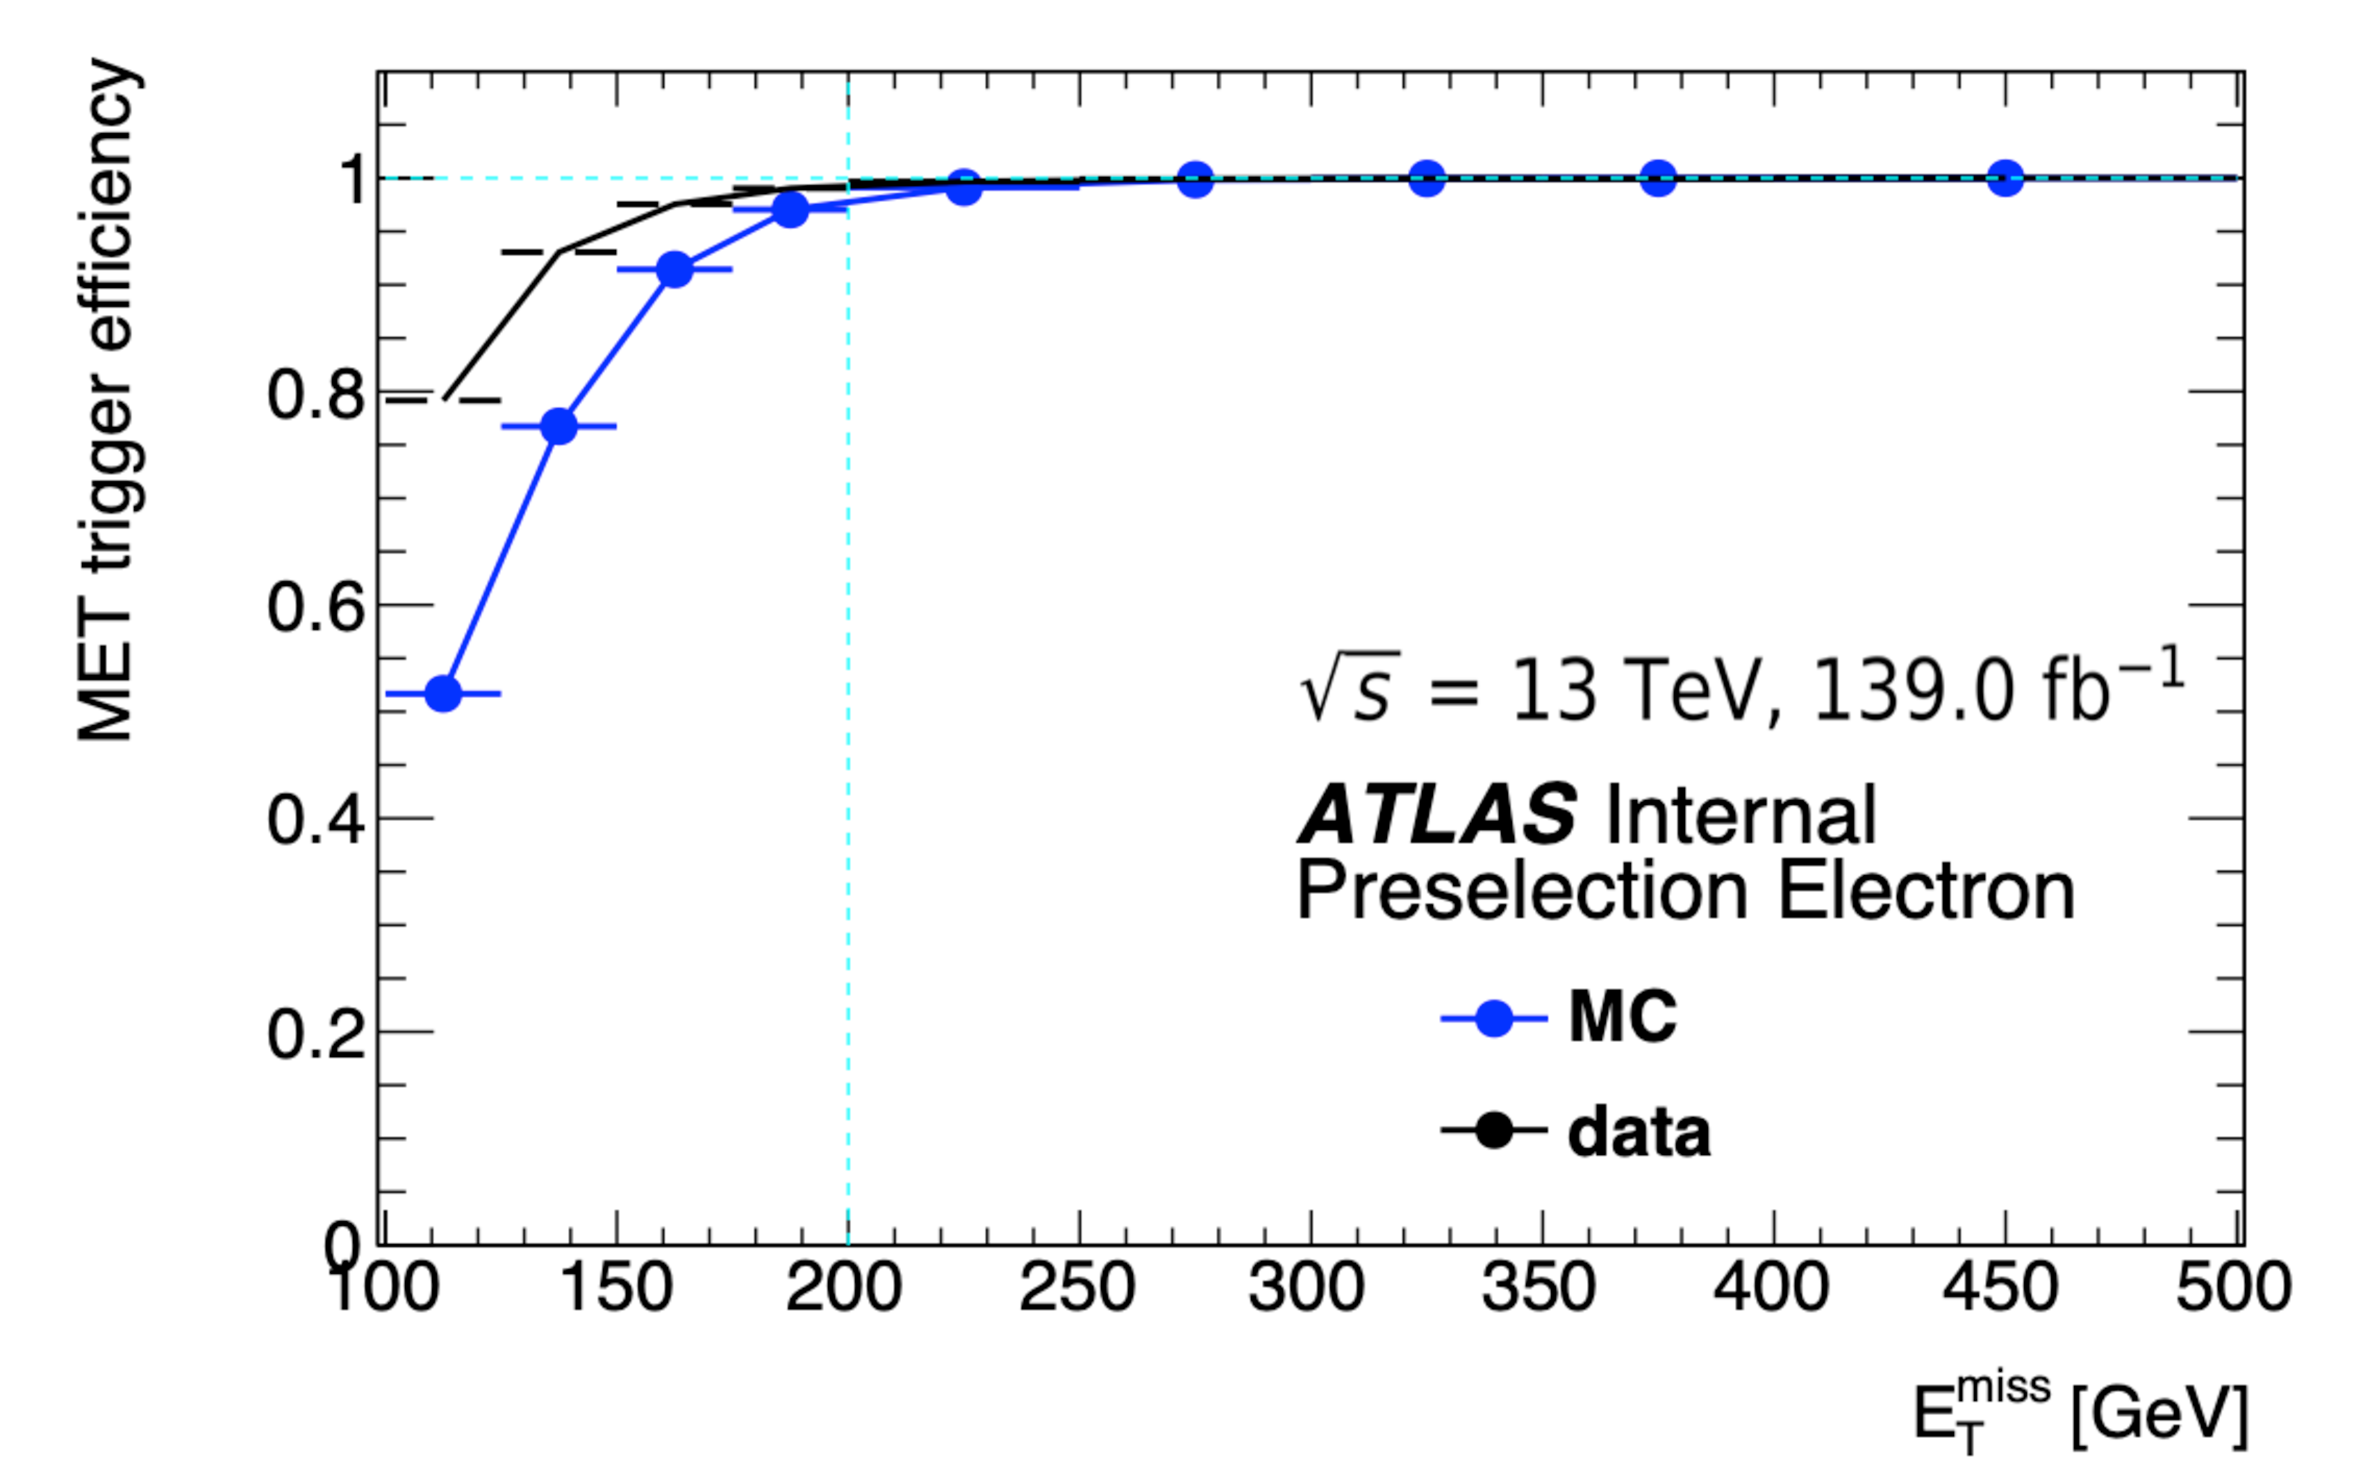
\includegraphics[width = 0.98\textwidth]{Figures/5/METTrigger/PreE_MetTST_met.pdf}
    \caption{Electron Channel}
    \label{ig:mettrig_e}
     \end{subfigure}
    \begin{subfigure}{0.49\textwidth}
     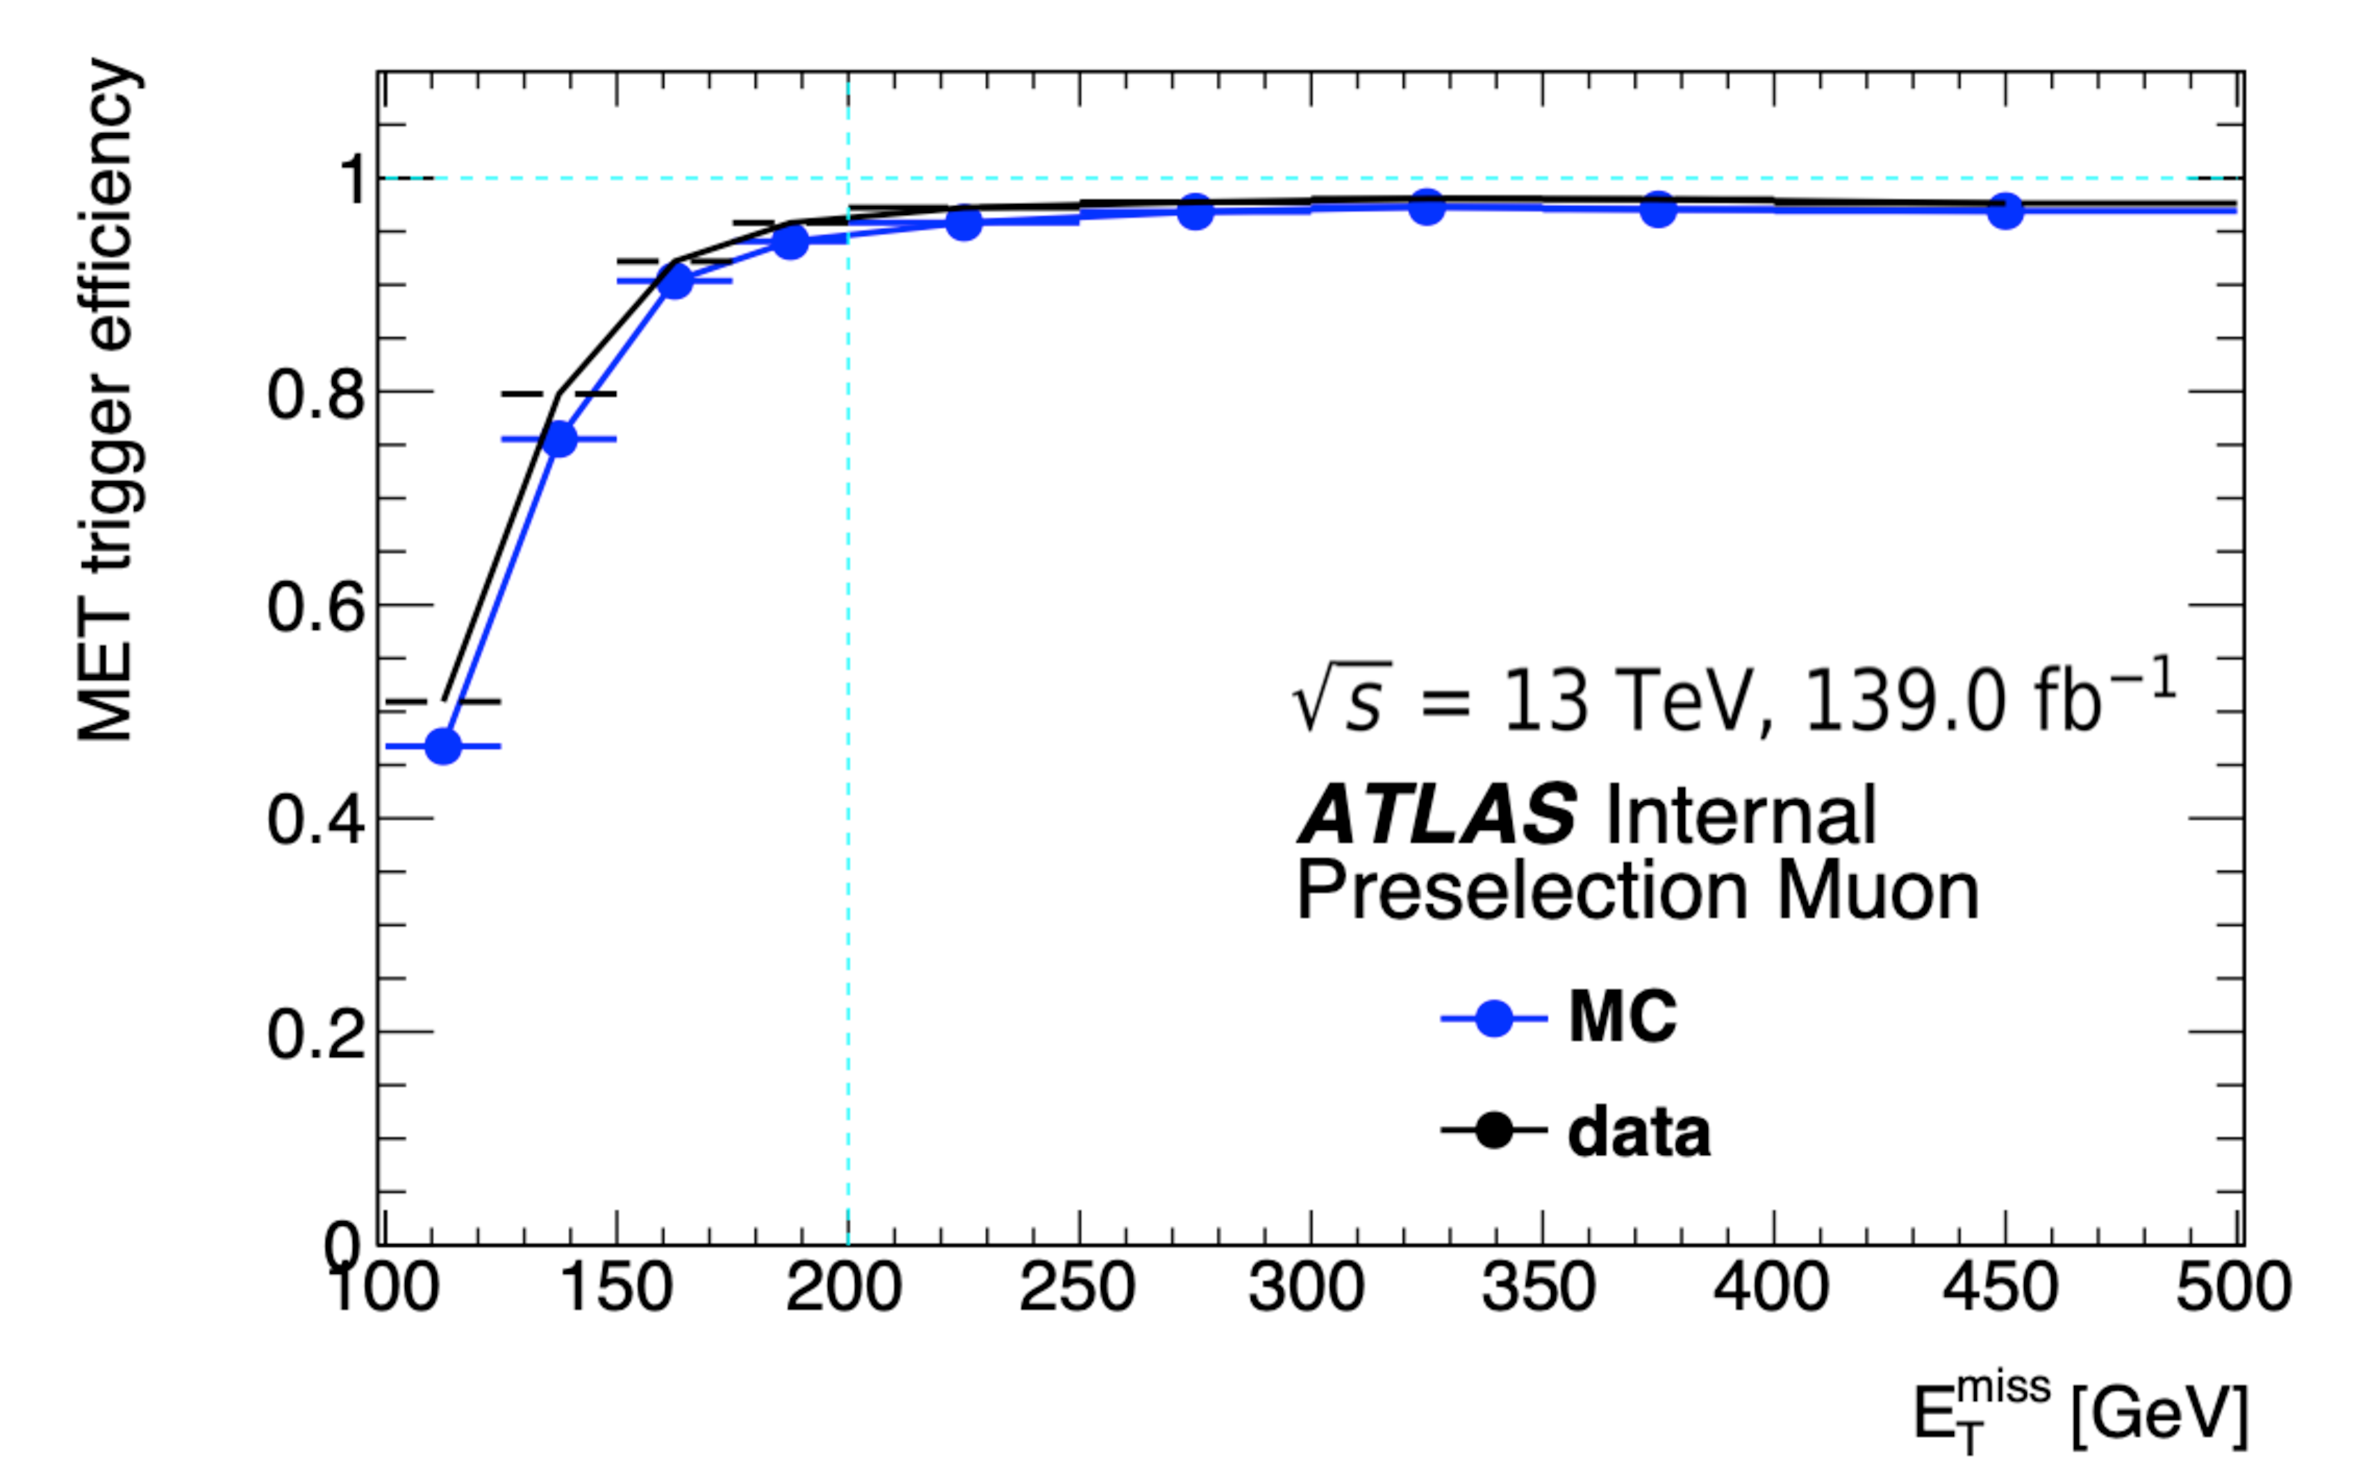
\includegraphics[width = 0.98\textwidth]{Figures/5/METTrigger/PreM_MetTST_met.pdf}
     \caption{Muon Channel}
     \label{ig:mettrig_mu}
     \end{subfigure}
     \caption{Comparison of the \met trigger efficiency defined in Eq. \ref{eq:met_trig_eff}, as a function of the \met lower bound in the event selection, between MC simulated events and ATLAS data in a region defined by a loosened baseline selection. The event selection is separated into electron (left) and muon (right) channels.}
     \label{fig:mettrig}
  \end{figure}
  
Comparing the trigger efficiencies in Figures \ref{fig:mettrig_e} and \ref{fig:mettrig_mu}, the efficiency in the electron channel converges to 100\% for \(\met > 200~\GeV\), but in the muon channel it instead converges to \(\sim90\%\) for \(\met > 200~\GeV\). After some investigation, the inefficiency in the muon channel was found to be due to events which have large \met arising from high-\pt muons. This is because high-\pt muons largely pass through the ATLAS calorimeter and are detected instead by the muon spectrometer. As a result, such high-\pt muon events can be missed by the \met triggers, which don't make use of information from the muon spectrometer \cite{met_performance_2019}. This can be seen by plotting the \met trigger efficiency using a calculation of \met in the event selection that ignores the muon \pt (a.k.a. ``muon invisible") in Figure \ref{fig:metmuinvis}, and observing that in this case the efficiency converges to 100\% for \met (muon invisible) \(> 200~\GeV\). 

\begin{figure}[htbp]
    \centering
     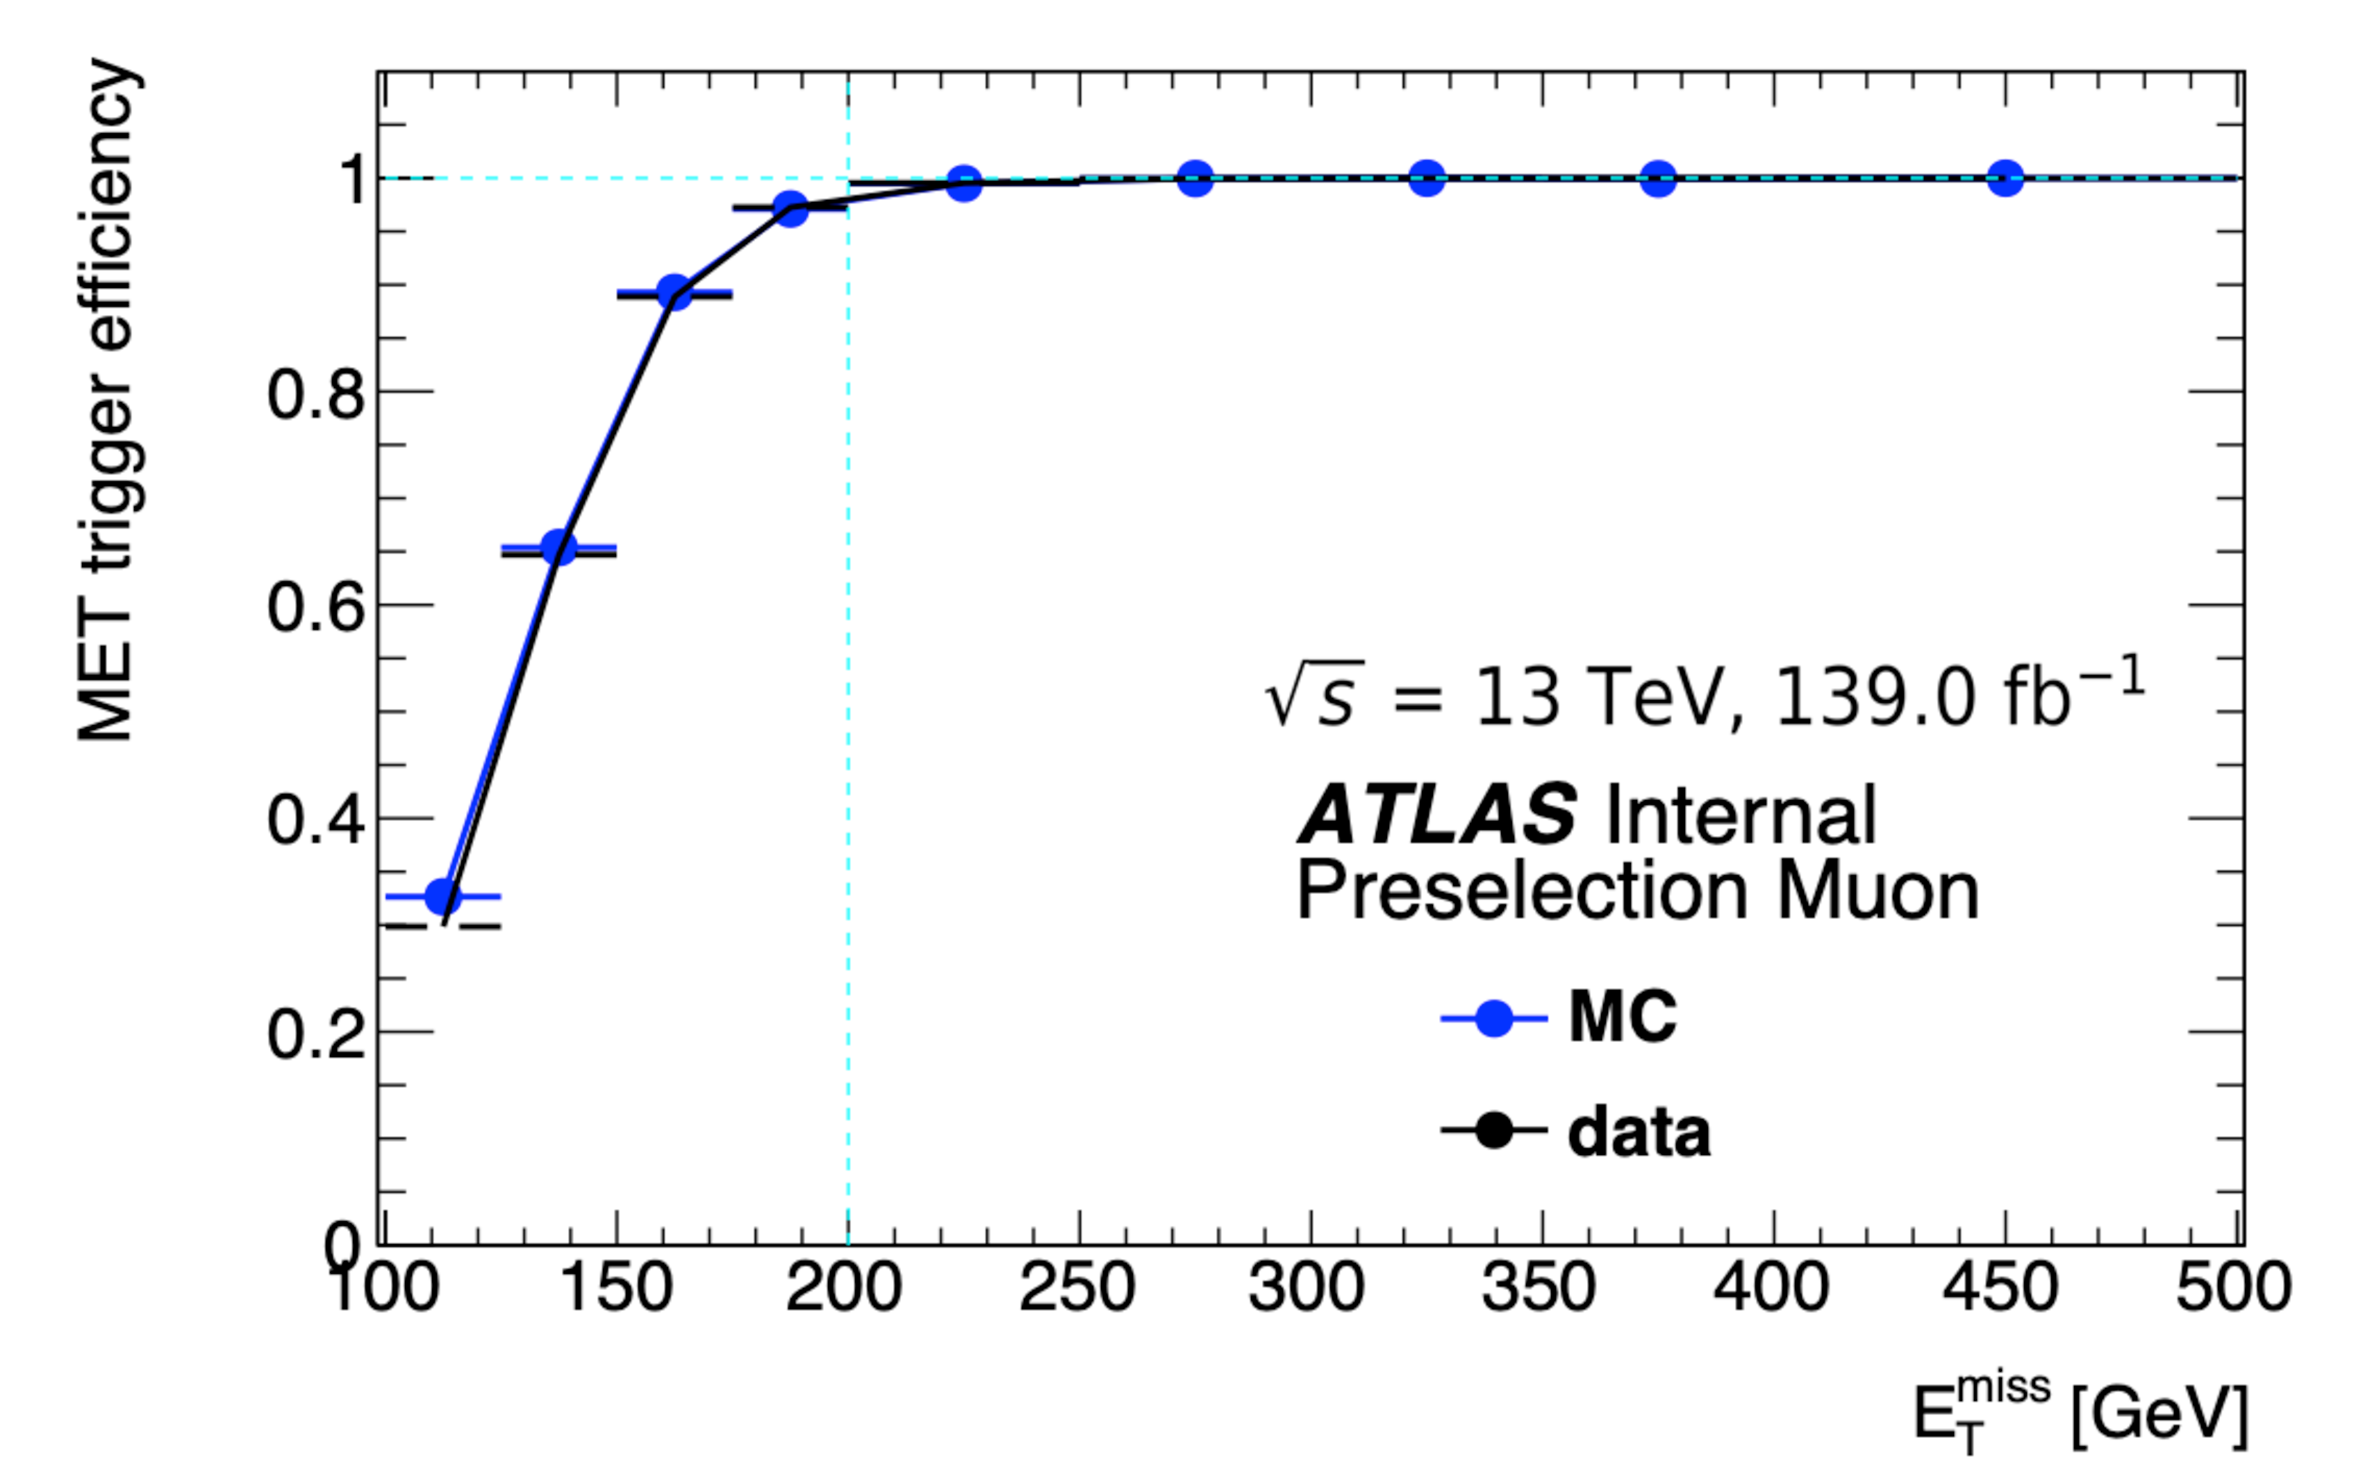
\includegraphics[width = 0.6\textwidth]{Figures/5/TriggerMuInvis/Pre_MetTST_met.pdf}
     \caption{\met trigger efficiency, as a function of the \met lower bound for the loosened baseline event selection in the muon channel, with muons treated as invisible in the calculation of \met}
     \label{fig:metmuinvis}
  \end{figure}
 
As discussed above, events which pass the baseline selection in the muon channel with \(\met > 200 ~\GeV\) but fail the \met trigger generally have large muon \pt. It was found that these high-\met events in the muon channel which fail the \met trigger do, however, pass the muon trigger with high efficiency. For this reason, the efficiency of a logical OR of the \met and single muon triggers is studied in the muon channel. This \met or single muon trigger efficiency is calculated as follows for MC simulated events for a given set of event selection criteria which define a region ``X":

\begin{equation}
\label{eq:met_or_single_muon_trig}
\begin{footnotesize}
\text{eff}_\text{\met OR single muon, MC, region X} = \frac{\sum_i w_i\text{ passing ($\met$ OR single muon triggers)\text{ AND }(in region X)}}{\sum_i w_i\text{ in region X}}
\end{footnotesize}
\end{equation}

\noindent where the event weight \(w_i\) in the numerator includes the scale factors to correct for the known \(<100\%\) trigger efficiency of the single muon trigger. Note that since Eq. \ref{eq:met_or_single_muon_trig} is evaluated only for MC simulated events, there is no need for an independent trigger in the numerator and denominator such as the single lepton trigger included in Eq. \ref{eq:met_trig_eff}. As shown in Figure \ref{fig:trigger_OR}, the \met OR single muon trigger is found to be effectively 100\% efficient, given the application of appropriate scale factors for the single muon trigger, in the muon channel with the loosened baseline event selection for all lower bounds on the \met down to  \(\sim 100~\GeV\).

  \begin{figure}[htbp]
  \centering
    \begin{subfigure}{0.49\textwidth}
     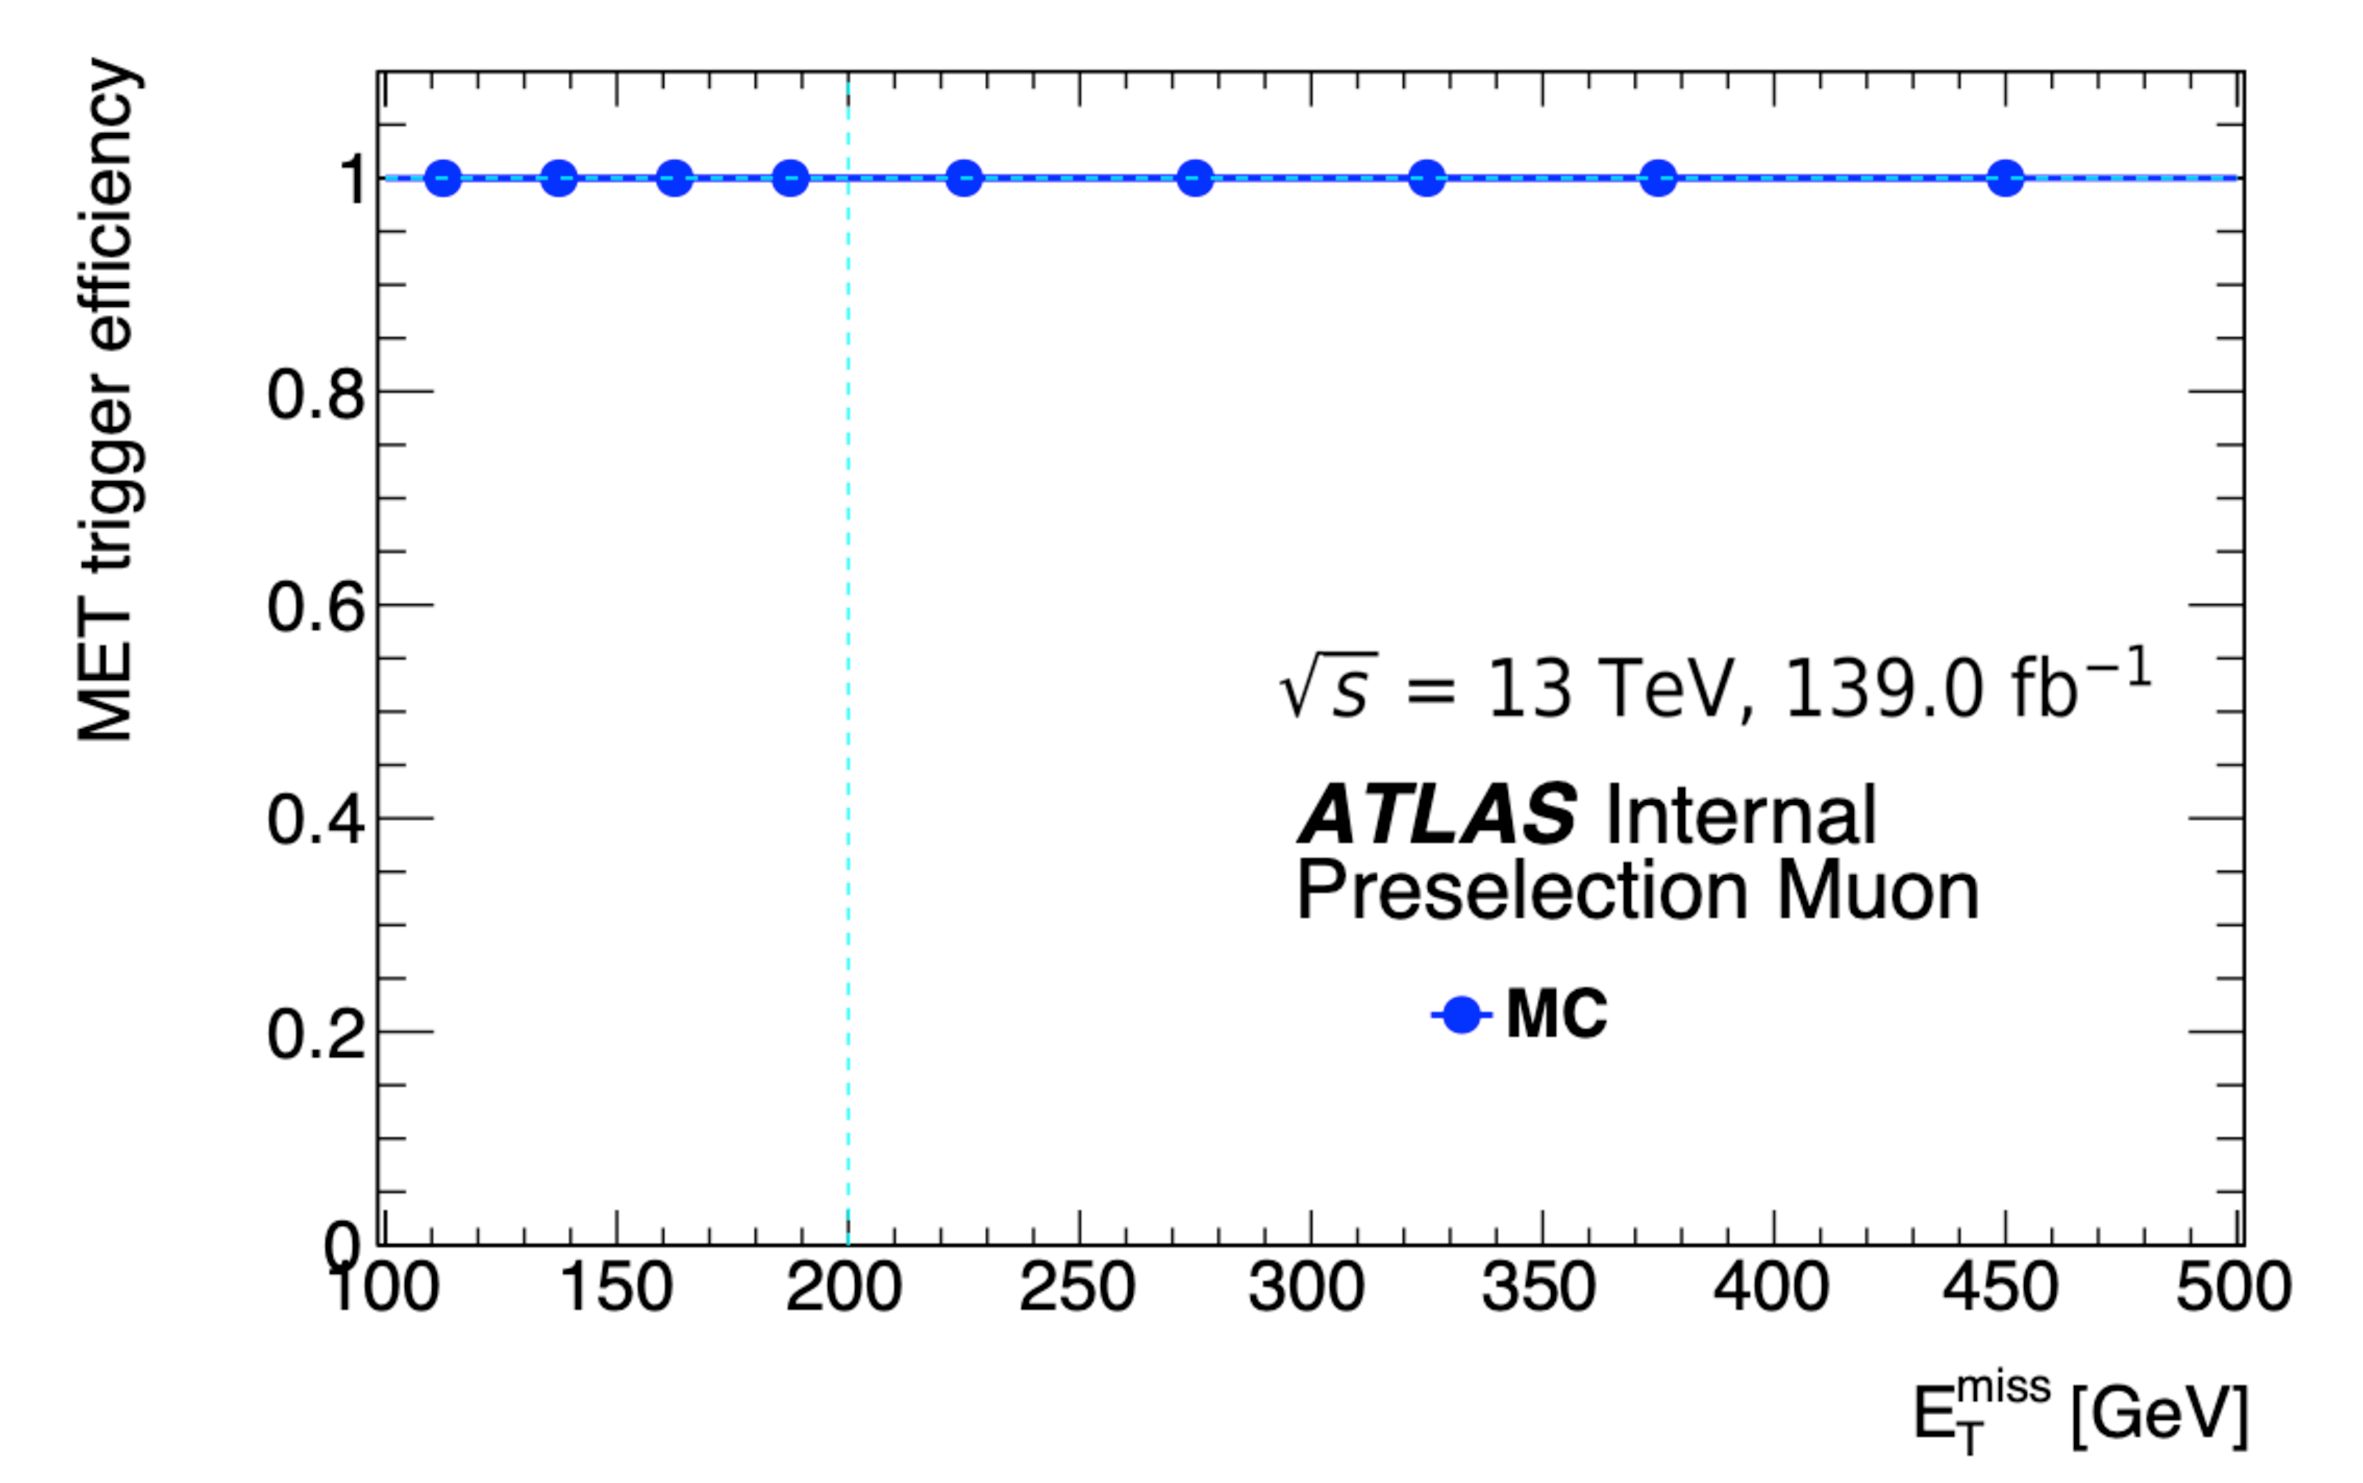
\includegraphics[width = 0.98\textwidth]{Figures/5/TriggerOR/Pre_MetTST_met.pdf}
     \caption{Preselection}
     \end{subfigure}
     \caption{Efficiency of the \met OR single muon trigger, as a function of the \met lower bound, in the muon channel for the loosened baseline event selection in the muon channel.}
     \label{fig:trigger_OR}
  \end{figure}

Based on the analysis presented in this section, it is concluded that, if all events considered in the analysis are explicitly required to have passed the \met or the single muon trigger, the trigger efficiency is known to be 100\% for all events except for the small subset of events with a high-\pt muon which pass the muon trigger but fail the \met trigger. For these events, scaling factors and associated uncertainties, which are determined by independent calibrations performed by the ATLAS collaboration, are included in the event weight to correct for the known \(<100\%\) efficiency of the single muon trigger. An additional ``trigger-matching" requirement is applied for events which fail the \met trigger but pass the single muon trigger. This trigger matching requires that the final state muon object that was reconstructed during data-taking and which activated the single muon trigger can be identified as the same muon object (i.e. as having originated from the same muon) that was later reconstructed with the more granular offline reconstruction software. 
